\documentclass[a4paper, twoside, 11pt]{report}
\linespread{1.1}
%% Language and font encodings
\usepackage[english]{babel}
\usepackage[utf8x]{inputenc}
\usepackage[T1]{fontenc}

%% Sets page size and margins
\usepackage[a4paper,top=3cm,bottom=2cm,left=3cm,right=3cm,marginparwidth=1.75cm]{geometry}

%% Useful packages
\usepackage{amsmath}
\usepackage{subfig}
\usepackage{graphicx}
\setlength {\marginparwidth }{2cm}
\usepackage[colorinlistoftodos]{todonotes}
% \usepackage[colorlinks=true, allcolors=blue]{hyperref}
\usepackage{hyperref}
\usepackage[capitalize]{cleveref} 
\usepackage[numbers]{natbib}
\usepackage{pgfgantt}
\usepackage{ltablex}
\usepackage{multirow}
\usepackage{color, colortbl}

% \usepackage{tikz}
% \usepackage{pgfplots}

\usepackage{listings}
\crefname{lstlisting}{listing}{listings}
\Crefname{lstlisting}{Listing}{Listings}
\usepackage{xcolor}

\definecolor{codegreen}{rgb}{0,0.6,0}
\definecolor{codegray}{rgb}{0.5,0.5,0.5}
\definecolor{codepurple}{rgb}{0.58,0,0.82}

\lstdefinestyle{mystyle}{ 
    commentstyle=\color{codegreen},
    keywordstyle=\color{magenta},
    numberstyle=\tiny\color{codegray},
    stringstyle=\color{codepurple},
    basicstyle=\ttfamily\fontsize{8}{8}\selectfont,
    breakatwhitespace=false,         
    breaklines=true,                 
    captionpos=b,                    
    keepspaces=true,                 
    numbers=left,                    
    numbersep=5pt,                  
    showspaces=false,                
    showstringspaces=false,
    showtabs=false,                  
    tabsize=2,
    xleftmargin=.12\textwidth
}

\lstset{style=mystyle}

\title{Data-driven Classification Methods for Event-driven Cameras}
\author{Tejas Dandawate}
% Update supervisor and other title stuff in title/title.tex

\begin{document}
\begin{titlepage}

    \newcommand{\HRule}{\rule{\linewidth}{0.5mm}} % Defines a new command for the horizontal lines, change thickness here

    %----------------------------------------------------------------------------------------
    %	LOGO SECTION
    %----------------------------------------------------------------------------------------

    % 
\includegraphics[width=8cm]{title/logo.eps}\\[1cm] % Include a department/university logo - this will require the graphicx package

    %----------------------------------------------------------------------------------------

    \center % Center everything on the page

    %----------------------------------------------------------------------------------------
    %	HEADING SECTIONS
    %----------------------------------------------------------------------------------------

    \textsc{\LARGE MEng Individual Project}\\[1.5cm] % Name of your university/college
    \textsc{\Large Imperial College London}\\[0.5cm] % Major heading such as course name
    \textsc{\large Department of Electrical and Electronic Engineering}\\[0.5cm] % Minor heading such as course title

    %----------------------------------------------------------------------------------------
    %	TITLE SECTION
    %----------------------------------------------------------------------------------------
    \makeatletter
    \HRule \\[0.4cm]
    { \huge \bfseries \@title}\\[0.4cm] % Title of your document
    \HRule \\[1.5cm]

    %----------------------------------------------------------------------------------------
    %	AUTHOR SECTION
    %----------------------------------------------------------------------------------------

    \begin{minipage}{0.4\textwidth}
        \begin{flushleft} \large
            \emph{Author:}\\
            \@author % Your name
        \end{flushleft}
    \end{minipage}
    ~
    \begin{minipage}{0.4\textwidth}
        \begin{flushright} \large
            \emph{Supervisor:} \\
            Prof. Pier Luigi Dragotti \\[1.2em] % Supervisor's Name
            \emph{Second Marker:} \\
            Prof. Patrick A. Naylor % second marker's name
        \end{flushright}
    \end{minipage}\\[2cm]
    \makeatother

    % If you don't want a supervisor, uncomment the two lines below and remove the section above
    %\Large \emph{Author:}\\
    %John \textsc{Smith}\\[3cm] % Your name

    %----------------------------------------------------------------------------------------
    %	DATE SECTION
    %----------------------------------------------------------------------------------------

    {\large \today}\\[2cm] % Date, change the \today to a set date if you want to be precise

    \vfill % Fill the rest of the page with whitespace

\end{titlepage}

\renewcommand{\abstractname}{Final Report Plagiarism Statement}
\begin{abstract}
    I affirm that I have submitted, or will submit, an electronic copy of my final year project report to the provided EEE link.

    I affirm that I have submitted, or will submit, an identical electronic copy of my final year project to the provided Blackboard module for Plagiarism checking.

    I affirm that I have provided explicit references for all the material in my Final Report that is not authored by me, but is represented as my own work.
\end{abstract}

\renewcommand{\abstractname}{Acknowledgements}
\begin{abstract}
    Firstly, I would like to thank Prof. Pier Luigi Dragotti for the opportunity to undertake this project under his supervision. He gave me a lot of much needed guidance throughout the process, while still affording me the freedom to take the project where I saw fit.

    I would also like to extend my gratitude to my family, without whom I would not be in this position, for which I will be forever in their debt. And finally, to my friends who have been instrumental in keeping me sane through these four long years - thank you all.
\end{abstract}

\renewcommand{\abstractname}{Abstract}
\begin{abstract}
    Neuromorphic sensing is a novel way of encoding analogue signals, inspired by the biological processing of information in our brains. Neuromorphic sensing is based on time encoding, where rather than recording the amplitude of the input signal at predefined times, one records the time instants where the amplitude surpasses a certain trigger mark. This leads to a very efficient way of acquiring and processing signals.

    The main aim of the project is to utilise data retrieved from neuromorphic cameras to carry out video classification. Two pipelines are devised to achieve this; one involves directly classifying event data, while the other is a two-phase network were events are first reconstructed into intensity videos before classification is done. With both pipelines, a series of networks are used for classification in order to ensure there is a fair comparison.
    
    Data pre-processing is also a large part of the machine learning pipeline, and as such played a part in the creation of the two pipelines. For the direct-event classification pipeline in particular, varying pre-processing methods are used. In most neuromorphic data analyses a method called `frame integration' is utilised, where events are segmented into time bins and accumulated into frames. In the classical approach, each frame has two channels depicting whether a positive of negative event occurred in each pixel during a particular time bin. In this project, the classical implementation was used as well as a new novel approach. Multiple networks were designed and implemented to be a part of both classification pipelines. The main ones  were convolutional and recurrent neural networks. Finally, a fully neuromorphic system using a spiking neural network is devised, allowing for the exploitation of the sparse data communication between layers. With similar performance, these networks can be utilised for low-powered devices and real-time classification in future works.
\end{abstract}

\pagenumbering{gobble}

\tableofcontents
\listoffigures
\listoftables \thispagestyle{empty}

\pagenumbering{arabic}

\chapter{Introduction} \setcounter{page}{1} \label{chap:introduction}
% The introduction should set the scene and give a high-level problem statement/specification, so that after 
% reading the introduction the reader understands
% roughly what the problem is and what you intend to 
% do about it. Is the idea to write software, or develop 
% an algorithm, or produce hardware, or something 
% else?
% You should then highlight and summarise the most 
% interesting or important questions or problems that 
% your project addresses, and the broader context in 
% which those questions or problems are situated.
% Finally, you must briefly introduce the structure of 
% report (what you will cover in which chapters and how 
% these relate to each other). You don’t need to go into 
% any detail, the aim is to make sure the reader has an 
% idea about what will be discussed and in what order.

\section{Motivations}

Neuromorphic data is obtained from event-based cameras that differ from traditional frame-based cameras in that each pixel asynchronously record `events', which are categorised as large shifts in light intensity. This is a novel representation of data that has overarching benefits that are yet to be fully explored in a plethora of applications. Event-based cameras have the potential to revolutionise efficient, low-power computer vision due to their efficient encoding of information. Since the cameras are asynchronous in nature they allow for low-latency feeds with very little motion blur and other similar visual artefacts. As well as this their pixel structure allows for a very high dynamic range, meaning they can be used even when bright sunlight and dark shadows are encompassed in the same scene.

With the emergence of the Internet of Things (IoT), sensors have become, or at the very least will become, ubiquitous in everyday life. These devices operate using power at a premium since they need to perform adequately with a limited power supply (e.g., small battery cells etc.). This scarcity is further emphasised when attempting to do more power-intensive tasks. One such task is computer vision, which is becoming evermore prevalent as a means of human-computer interaction. Classical frame-based cameras are power intensive, and do not allow for a low active duty cycle (i.e., allowing for device sleep/idle time). The usual way in which this issue is alleviated is by making the system react to an event trigger by `waking up' to work for a short period of time. Such events may include things such as; motion, timing, acceleration, or temperature. When compared to the function of event-based cameras, where event detection is built into the system, this can be seen as a stop-gap measure. To further leverage the low power-consumption of event-based cameras, spiking neural networks could also be implemented to create a fully neuromorphic pipeline. The added benefit of such a system would be the ability to utilise the sparse data communication between spiking neurons, allowing for even greater power-efficiency for low-powered devices and real-time data analysis.

The high temporal resolution and dynamic range of event-based cameras also presents further benefits when compared to frame-based cameras. These features allow for videos to be represented in a very high fidelity format that preserves more data in fast-paced and brightly lit environments. This may lead to more reliable use of the data for computer vision and even other purposes where the exact environment the camera is set up in is uncertain and unpredictable.

\section{Problem Specification}

The problem this report tries to address is the processing of event-based data in order to employ commonly used computer vision algorithms. This is an exploratory venture into the field, and so the subsection of classification problems was chosen. 

Most commonly used classification models have been designed with inputs from frame-based cameras in mind. For this reason, a novel approach was designed wherein event streams are first converted into intensity videos using pre-built and trained models such as the E2VID reconstruction model\cite{spikingToVideo}, which can then be fed into pre-existing classification models. This two-phase pipeline can then be compared with classification directly on event data.

% To ensure a fair comparison of the two methods, the same networks were applied to the outputs so that there were no extraneous factors effecting their performance. 

Additionally, in the field of event analysis, a method known as frame-integration is commonly applied, which allows for the construction of frames from segments of event data. This method allows for the implementation of custom integration techniques, which could improve the performance of the direct event classification pipelines.

Finally, there is growing interest in spiking neural networks, since they have sparse data communications between neurons. This means that they are more suited for efficient data transfer and fast inference than artificial neural networks. A large benefit of frame-based cameras and their data representations is the energy efficiency, lending itself to use in low-powered devices. The investigation of novel spiking neural networks would allow for a fully neuromorphic system, which could be tested in future work for low-power devices and real-time inference.

\section{Requirements Capture} \label{sec:requirements_capture}

% Projects with a deliverable that serves a specific 
% function often have an initial phase in which expected 
% use is investigated and a brief more detailed than the 
% specification is constructed. This would include what 
% is necessary, what is desirable, etc in the final 
% deliverable. The results of requirements capture 
% determine project objectives and are used to inform 
% project evaluation.
% Requirements capture is important in all projects with 
% real-world deliverables, and is often a significant 
% amount of work in software projects. Where 
% requirements capture is less relevant (for example in
% an analytical ‘research-style’ project) this may be 
% replaced by a detailed description of the project aims 
% and objectives in the Introduction or the Background 
% sections.

\begin{itemize}
      \item Load and prepare neuromorphic datasets for use in the project.
      \item Process data and set-up pipeline for two-phase intensity reconstruction and classification.
      \item Process data and set-up pipeline for direct event analysis.
      \item Create various classification models to act as a basis of comparison between two classification pipelines.
      \item Create spiking versions of classification models with similar classification accuracies.
      \item Create evaluation plan with detailed metrics to compare both the performance of the two pipelines, as well as the individual classification models used in each.
      \item Compare and contract findings to understand best ways to discern most appropriate event-driven analysis method.
\end{itemize}

\section{Report Structure}

A brief outline of the report is given below:

\begin{description}
      \item[Background] (\Cref{chap:background})

            This chapter gives a background to the project subject. There are outlines of previous works in the field in order to highlight gaps in knowledge where more work can be done. It provides a good illustration of what issues there are and what value there would be in solving them.
      % \item[Implementation Plan] (\Cref{chap:implementation_plan})

      %       This chapter has a list of planned objectives and their estimated completion date.
      % \item[Evaluation Plan] (\Cref{chap:evaluation_plan})

      %       This chapter presents a variety of ways in which the final project could be evaluated at each step. This allows for a comparison between existing solutions as well every iteration of solution created during the project.
      % \item[Ethical, Legal and Safety Plan] (\Cref{chap:ethical_plan})

      %       This chapter presents any ethical, legal and safety considerations taken into account during the project.

      \item[Analysis and Design] (\Cref{chap:analysis_and_design})
      
      In this chapter a high level overview of the design is given. This includes the choices of hardware/software, as well as architectural diagrams and descriptions.

      Additionally this chapter presents a variety of ways in which the final project was evaluated. This allows for a comparison between existing solutions as well every iteration of solution created during the project.

      \item[Implementation] (\Cref{chap:implementation})

      This chapter outlines noteworthy aspects of the implementation process, as well as a rationale for each step of the projects creation, including any reasons it deviated from the initial design.

      \item[Testing and Results] (\Cref{chap:testing_and_results})
      
      Following the evaluation plan in \cref{chap:analysis_and_design}, this chapter aims to apply the planned evaluation techniques to the performance of each of the pipelines and constituent networks. As well as this it includes reasoning for any interesting findings, acting as a basis for the overall evaluation of all implemented systems.

      \item[Evaluation] (\Cref{chap:evaluation})
      
      This chapter includes a critical evaluation of all systems implemented in the duration of the project. As opposed to the previous chapter, where details explanations of results and comparisons between classification models are given, this one appraises both pipelines in general, commenting on the effectiveness of event-stream classification. It also acts to measure the success of the project in terms of achieving the aims outlined in \cref{sec:requirements_capture}.
      
      \item[Conclusion and Further Work] (\Cref{chap:conclusion_and_further_work})
      
      This final chapter reports the overall success of the project, and outlines what has been achieved in general. As well as this the limits of the project are discussed, including further works that could act as an extension of the project to improve its effectiveness. Finally it includes a comment on the work from others in this field, including any similarities that have arisen between the work created in parallel to this project.
      
      \item[Appendices]
      
      Appendices including code-snippets, model architectures and details results tables.
\end{description}
\chapter{Background} \label{chap:background}

% You should provide enough background to the reader 
% for them to understand what the project is all about, 
% and what is the relevant prior work.
% Examiners like to know that you have done the 
% appropriate background research and it is important 
% that you review either what has been done previously 
% to tackle related problems, or perhaps what other 
% products exist related to your deliverable. Clear 
% references are important here, and much of this 
% section will typically already have been written in your 
% Interim Report. You may use feedback from that 
% report to improve what you write in your Final Report, 
% and should note that self-plagiarism between the two 
% reports is not possible, so no citation is needed of 
% your own earlier writing.

%  What does the reader need to know in order 
% to understand the rest of the report? What 
% problem are you solving?
%  Why is this problem interesting or worthwhile 
% to solve?
%  Who cares if you solve it?
%  How does this relate to other work in this 
% area?
%  What work does it build on?
%  For 'research-style' projects involving the 
% design and analysis of specific algorithms 
% there is a large amount of relevant 
% background both of general theory, and very 
% specific to the algorithm you investigate. 
% Supervisors will help you to see what is most 
% important here, but the general rule is that 
% you must both provide overall context and 
% note work close to what you do that 
% influences your work or is in some way 
% comparable to your work.

This chapter outlines background information required for understanding the basis for the project. The theory and literature serves to outline the main concepts used for neuromorphic data processing, as well as to reveal gaps in existing research that require solidifying.

\section{Event Cameras}

Event based cameras can be described as `bio-inspired sensors that differ from conventional frame cameras: Instead of capturing images at a fixed rate, they asynchronously measure per-pixel brightness changes, and output a stream of events that encode the time, location and sign of the brightness changes' \cite{EventBasedVisionASurvery}.

\subsection{Benefits} \label{ssec:event_camera_benefits}
Event-based cameras are purported to provide a number of benefits including;

\begin{itemize}
      \item \textbf{High temporal resolution}

            The reason for this is that whereas frame-based cameras have a certain frame-rate, event-based cameras do not have this limitation, meaning the "blind time" between frames is eliminated. The reason for this is that the function of a frame-based camera is dependent on the global shutter to capture the light at a particular instant, whereas event-based cameras can be thought of as having individual shutters for each pixel that are shut whenever an event occurs.
      \item \textbf{High dynamic range}

            The reason for this is again the fact that each pixel has its own individual shutter, but as well as this they all use a logarithmic scale, meaning they function well from very bright to very dim environments as well as fast shifts between the two.
      \item \textbf{Low power consumption}
      \item \textbf{High pixel bandwidth}

            Each pixel can capture events at the rate of ~kHz. This has the effect of reducing blur since there is a very high temporal resolution to begin with. This makes the system very responsive and therefore ideal for real-time systems.
      \item \textbf{Efficient Encoding}

            Since events are asynchronous and spatially sparse (i.e there are mainly 0 values in the output matrix), the encoding is very efficient, as opposed to frame-based cameras that produce data that is very spatially dense.
\end{itemize}

The above benefits are very persuasive reasons to adopt neuromorphic cameras in many different applications. It is conceivable that if algorithms can make use of these benefits (since most classical algorithms play to the strengths of the data generated by frame-based cameras), real-time systems could be completely revolutionised.

\subsection{Function} \label{ssec:event_camera_function}
Event-based cameras differ from frame based cameras fundamentally, in that they do not rely on a global shutter closing at regular intervals to record information of a scene. Instead each pixel closes whenever it detects an `event' occurring. The way such events are detected is dictated by the `event generation model'\cite{EventBasedVisionASurvery}.

Each pixel responds to changes in its log photo-current ($ L = log(I) $, where $I$ is the perceived brightness), giving the system a very high dynamic range. A recorded event `$ k $' has the format $ e_k = (\boldsymbol{\mathbf{x}}_k, t_k, p_k ) $. This is known as the Address Event Representation (AER). The first value is the spacial location of the event ($ \boldsymbol{\mathbf{x}}_k = (x_k, y_k)^\top $), the second value $ t_k $ is the temporal location, and the final value $ p_k \in {1, -1} $ indicates the polarity of the event (i.e in which direction the brightness gradient was changing). The brightness increment between two events at the same pixel is given by the equation $ \Delta L(\boldsymbol{\mathbf{x}}_k, t_k) = L(\boldsymbol{\mathbf{x}}_k, t_k) - L(\boldsymbol{\mathbf{x}}_k, t_k - \Delta t_k) $. In a perfect (noise free) environment an event is fired whenever the brightness increment reaches a temporal contrast threshold. This relationship is shown in \cref{eq:ideal_event_equation}.

\begin{equation}
      \Delta L(\boldsymbol{\mathbf{x}}_k, t_k) = p_k C ( C > 0 )
      \label{eq:ideal_event_equation}
\end{equation}

It should be noted that the value of $ C $ could be variable and therefore different for $ p_k = \pm 1 $. Additionally, we can approximate the temporal derivative of a pixels brightness by substituting \cref{eq:ideal_event_equation} into the Taylor expansion given in \cref{eq:temporal_derivative_taylor_exp}. \cref{eq:temporal_derivative} shows the resulting format for the temporal derivative.

\begin{equation}
      \Delta L(\boldsymbol{\mathbf{x}}_k, t_k) \approx \frac{\delta L}{\delta t}(\boldsymbol{\mathbf{x}}_k, t_k)\Delta t_k
      \label{eq:temporal_derivative_taylor_exp}
\end{equation}

\begin{equation}
      \frac{\delta L}{\delta t}(\boldsymbol{\mathbf{x}}_k, t_k) \approx \frac{\Delta L(\boldsymbol{\mathbf{x}}_k, t_k)}{\Delta t_k} = \frac{p_k C}{\Delta t_k}
      \label{eq:temporal_derivative}
\end{equation}

It should however be noted that the approximation in \cref{eq:temporal_derivative_taylor_exp} is only true under the assumption that $ \Delta t_k $ is exceedingly small. Since unlike frame-based cameras we do not measure absolute brightness, this is an indirect way of measuring and keeping track of the brightness within the frame.

\cref{fig:davis_camera} shows the basic functionality of an event-based camera. Shown in \textbf{(a)} is the simplified circuit diagram of the DAVIS pixel, which in \textbf{(b)} is used to convert light into events (shown in real life in images \textbf{(c)} and \textbf{(d)}). \textbf{(e)} shows how this setup would view a white square rotating on a black disk. It is a stream of events going from the past in green to the present in red. These events can then be seen overlaid on a natural scene in \textbf{(f)}.

\begin{figure}[htb]
      \centering
      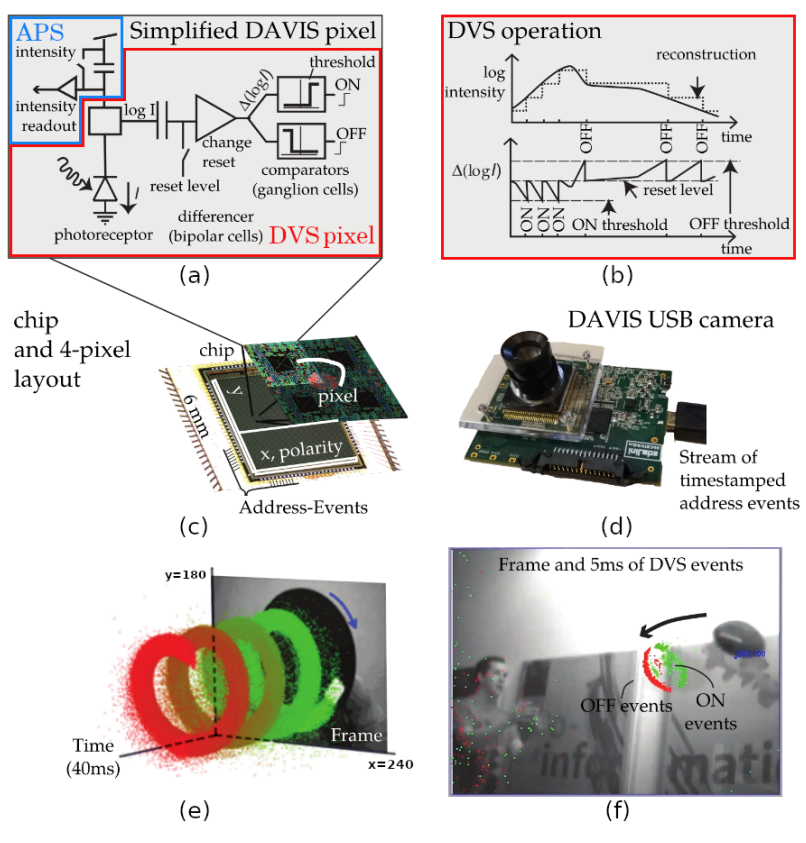
\includegraphics[width=0.5\textwidth]{background/images/davis_camera.png}
      \caption{A summary of the functionality of the DAVIS event based camera\cite{EventBasedVisionASurvery}.}
      \label{fig:davis_camera}
\end{figure}

\section{Spiking Neural Networks and Neural Heterogeneity} \label{ssec:snn_and_heterogeneity}

\Cref{ssec:event_camera_benefits} lists some persuasive reasons for utilising neuromorphic systems, but there still many challenges posed when attempting to do so. For example, each pixel only responds to brightness change, but the problem is that such a change could be a result of not only scene changes, but also the position of the camera within the scene. For this reason most neuromorphic systems have currently been limited to stationary cameras. As well as this, the system is especially prone to stochastic noise due to inherent shot noise in photons and from transistor circuit noise \cite{EventBasedVisionASurvery}. For this reason \cref{eq:ideal_event_equation} can only be said to be true under ideal conditions. A more realistic model for events fired is a probabilistic event generation model. These take into consideration the aforementioned sources of noise. One such model is given by P. Lichtsteiner \textit{et al.}\cite{NonIdealEventCamera}, where sensor variation measurements suggested a normal distribution centred around $ C $ for event triggers.

In order to tackle issues such as the ones due to noise, it is useful to look at existing examples of spiking neural systems, such as a biological brain. It is known that the brain is heterogeneous on every scale, in the past this was thought to be simply a by-product of noisy processes, but more recently it can be shown that by adding heterogeneity to Spiking Neural Networks (SNNs), a more stable and robust system can be created\cite{NeuralHetroPromRobLearn}, indicating this heterogeneity has a more deep rooted purpose. As well as this the learned neural parameters tend to resemble what can observed experimentally. This may serve as an explanation for how the brain has evolved to deal with the many stochastic processing it encounters.

The foundations of SNNs are in computational neuroscience. The mechanisms of neurons in the brain are the inspiration behind creating ANNs with neurons that spike in the same way. Neurons in an a typical ANN have a weight, bias and activation function. This means that the output of the neurons can be summarised by \cref{eq:artificial_neuron_output}.

\begin{equation}
      y = \theta(\sum^n_{j=1}w_jx_j-u_j)
      \label{eq:artificial_neuron_output}
\end{equation}

This model was inspired by the biological neuron model shown in \cref{fig:biological_neuron}. The function of the neuron is similar in that it produces an output based on a function of the input stream, but the form of this output is in the form of a `spike' rather than a continuous function. The $ \Sigma $ shown in the diagram is actually the integration of all excitory and inhibitory input signals to the dendrites coming from the soma of the neuron. We can see that the electric potential of the neuron needs to exceed a certain threshold in order for the output of the neuron to be a spike. Spiking neural networks use a similar model of neurons in order to leverage the aforementioned benefits of neural heterogeneity.

\begin{figure}[htb]
      \centering
      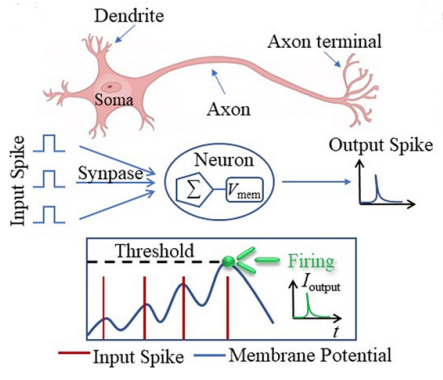
\includegraphics[width=0.4\textwidth]{background/images/biological_neuron.png}
      \caption{A diagram of structure and function of a biological neuron \cite{BiologicalNeuronModel}.}
      \label{fig:biological_neuron}
\end{figure}

With SNNs it is theoretically possible to achieve very high energy efficiency, and when combined with a novel surrogate gradient and Recurrent Neural Network (RNN) as was experimented with in a paper by Bojian Yin \textit{et al.}\cite{EfficientSNN} excels in challenging tasks such as gesture recognition, and at some points even outperforms traditional ANNs. Alongside the aforementioned neural heterogeneity to combat stochastic processes we can see substantial improvements in previous SNN performance.

\section{Nengo} \label{sec:nengo}

\color{red} TODO: Write about nengo here \color{black}.

\section{Existing Algorithms for Event Analysis} \label{sec:existing_algorithms}

For SLAM, pose estimation and classification tasks the problem again is that classical systems heavily rely on the structure of conventional camera's outputs, and so there needs to be a radical paradigm shift in order to take events as inputs instead.

\subsection{Optic-flow Methods}

Since obtaining the equation for the temporal derivative in \cref{eq:temporal_derivative}, there is now a indirect measure of brightness and so a more classic computer vision techniques using optic-flow constraints can be utilised to characterise the events detected by pixels. In frame-based systems, optic flow methods create a flow-field that describe the displacement vector (signifying direction and magnitude of movement) for each pixel in the frame, and a similar derivation can be done for event data. A core constraint in this derivation is that the intensity of a local time-varying image region is constant under motion (for at least a short amount of time)\cite{GenerativeEventModel}. \cref{eq:optic_flow} is the resulting equations that shows the relation between the brightness gradient and the displacement of the pixel over a short period of time given its velocity\cite{EventBasedVisionASurvery}. It implies that if the motion is parallel to the edge, there is no event fired (since $ v \cdot \nabla L = 0  $) and conversely if the motion is perpendicular to the edge events are fired at their highest rate.

\color{red} TODO: Write about how optic flow is often used in classification to see in a frame what the directions of motion are as well as the frame itself and the laplacian or edge map. \color{black}

\begin{equation}
      \Delta L \approx -\nabla L \cdot v \Delta t_k
      \label{eq:optic_flow}
\end{equation}

\subsection{Frame Integration of Event Streams}

A common method of getting frame-like videos from event data is to use the event-to-frame integration method. One such method is outlined by \textit{Wei Fang et al.}\cite{LearnableMembraneSNN}, which is the one used in the python package spikingjelly\cite{SpikingJelly}. The method used is outlined in \cref{eq:event_integration}.

Data in neuromorphic datasets are in the formulation of $ E(x_i, y_i, t_i, p_i) $ that represent the event's coordinate, time and polarity. We split the event's number $ N $ into $ T $ slices with nearly the same number of events in each slice and integrate events to frames. Note that $ T $ is also the simulating time-step. Denote a two channels frame as $ F(j) $ and a pixel at $ (p, x, y) $ as $ F(j, p, x, y) $, the pixel value is integrated from the events data whose indices are between $ j_l $ and $ j_r $:

\begin{align*}
      j_l = \lfloor \frac{N}{T} \rfloor \cdot j
\end{align*}
 
\begin{align*}
      j_r = \begin{cases}
            \lfloor \frac{N}{T} \rfloor \cdot (j + 1), & \text{if j < T - 1}\\
            N, & \text{if j = T - 1}\\
          \end{cases}
\end{align*}

\begin{equation}
      F(j, p, x, y) = \sum^{j_r -1}_{i=j_l}I_{p, x, y}(p_i, x_i, y_i)
      \label{eq:event_integration}
\end{equation}
 
where $ \lfloor . \rfloor $ is the floor operation, $ I_{p, x, y}(p_i, x_i, y_i) $ is an indicator function and it equals 1 only when $ (p, x, y) = (p_i, x_i, y_i) $.

\color{red} TODO: Write more about this method from the spikingjelly docs \color{black}

% \subsection{Localisation using Probabilistic Filters} \label{ssec:prob_filters}

% \subsubsection{Bayesian Inference}

% Unlike most other previous systems, probabilistic filters such as Bayesian filters are very much suited to work with data from event-based cameras. The reason for this is that it depends on iterative updates to the location probabilities using inputs, for which spiking inputs are ideal. Bayes's theorem can be derived from simple probabilistic rules\cite{BayesLaw}. We know $P(X|Y) = \frac{P(X, Y)}{P(Y)} $ and similarly $ P(Y|X) = \frac{P(Y, X)}{P(X)} $. Therefore we can re-arrange both to give $ P(X|Y)P(Y) = P(Y|X)P(X) $, since $ P(X, Y) = P(Y, X) $. Then from there formula for Bayesian inference can be trivially obtained, as shown in \autoref{eq:baysean_inference}.

% \begin{equation}
%       \begin{gathered}
%             P(XZ) = P(Z|X)P(X) = P(X|Z)P(Z)\\
%             P(X|Z) = \frac{P(Z|X)P(X)}{P(Z)}
%       \end{gathered}
%       \label{eq:baysean_inference}
% \end{equation}

% In \autoref{eq:baysean_inference}, $ X $ is known as the prior (which is the assumed location of the camera) and $ Z $ is known as the posterior (which is the measurement taken by the sensor or camera). $P(Z|X) $ is known as the likelihood function, which indicates how likely it is to have received a particular reading given the assumed position.

% \subsubsection{Monte-Carlo Localisation}

% Now that we have the concept of Bayesian inference we can adapt it to create an efficient localisation algorithm. It includes initialising a number of particles that act as predictors of where in the map the camera is. We can now give the probability of a posterior camera position given a sensor reading.

% The probability distribution $ P(X|X) $ is a continuous function, and so updating each of the posteriors for every value of $ X $ is a computationally difficult problem. We can instead break it up into smaller bins to alleviate this issue. When generating these particles we can represent the probability distribution, albeit at a lower granularity. The benefit of this is that even though we cannot see the full distribution the peaks (i.e. the locations the camera is most likely to be in) are very well defined.

% Now we can use the above simplification to carry out the following steps:

% \begin{enumerate}
%       \item Randomly assign particle distribution across map.
%       \item Apply Bayes' law to measurement to update particle distribution.

%             Bayes' rule can be simplified to be:
%             $$ w_{i_{x+1}} = P(z|x_{i_x}) \times x_{i_x} $$
%             This can be done since the ignored multiplier on the right hand side will be normalised in the next step.
%       \item Normalise particle weights.

%             Now the particles will have weights that no longer sum to 1, and so we need to normalise them again to follow the usual rules of probability:

%             $$ w_{i_{x+1}} = \frac{w_i}{\sum^N_{i=1}w_i} $$
%       \item Re-sample particle distribution.

%             We now need to create a new set of particles that all have the same weight ($ \frac{1}{N} $), but whose spacial distribution reflects the new probability density.
% \end{enumerate}

% \begin{figure}[htb]
%       \centering
%       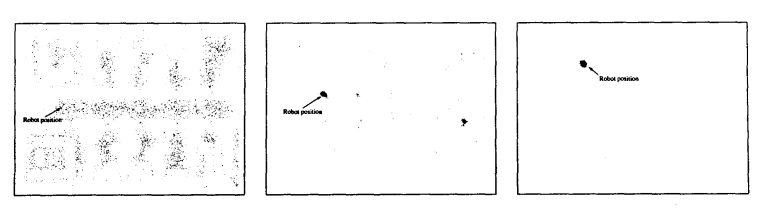
\includegraphics[width=\textwidth]{background/images/monte_carlo.png}
%       \caption{An example of Monte-Carlo localisation\cite{MonteCarloLocalisation}.}
%       \label{fig:monte_carlo}
% \end{figure}

% \autoref{fig:monte_carlo} shows a typical example of the algorithm. The leftmost panel shows the random initialisation (or previous particle distribution), which then becomes the centrally shown distribution after one iteration. Since only one measurement is taken and the room is symmetrical, it is possible that it could be in one of two location (hence the two dense clusters). After one more reading in the next iteration, the algorithm is quickly able to narrow down the location of the robot. We can also see that any movement of the robot causes some noise to be added to the known robot location as we are estimating the location based on simple odometry using hardware such as wheel encoders to estimate the robots motion.

% \subsection{SLAM Algorithm}

% The Monte-Carlo localisation technique is useful for estimating a vehicles position (i.e, its location and orientation) given a model (or map) of the environment surrounding it. The next step is to carry out pose estimation of a robot while simultaneously generating a map of its surroundings (as shown in \autoref{fig:slam_diagram}). It is clear from the diagram that the equipment is not perfect and in an idealised environment. There is uncertainty in both the robot position (since there is uncertainty in the robots odometry), and there is also uncertainty in the measurements the robot takes.

% \begin{figure}[htb]
%       \centering
%       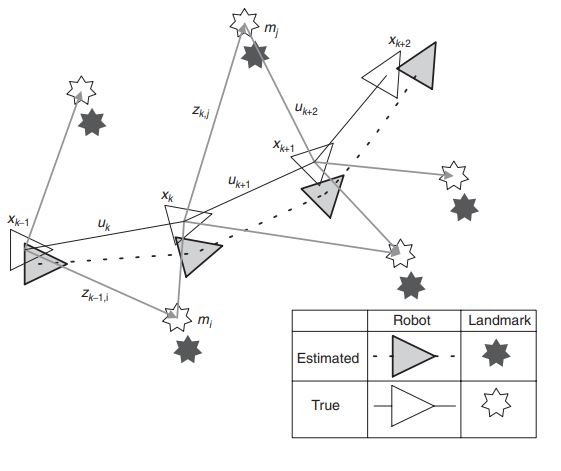
\includegraphics[width=0.4\textwidth]{background/images/slam_diagram.png}
%       \caption{A diagram showing the fundamentals of the SLAM problem\cite{BasicSlam}.}
%       \label{fig:slam_diagram}
% \end{figure}

% There are two main branches of SLAM algorithms; filtering methods and smoothing methods. The former includes methods such as the Extended Kalman Filter (EKF) and particle filtering (similar to the Monte-Carlo filtering explained earlier). With these methods the state is estimated iteratively on the job as latest measurements are input into the system. The latter uses the set of complete measurements to estimate the full trajectory of a robot. Pose (or factor) graph optimisation is one such smoothing method that has become exceedingly popular in modern-day SLAM solutions.

% \begin{figure}[htb]
%       \centering
%       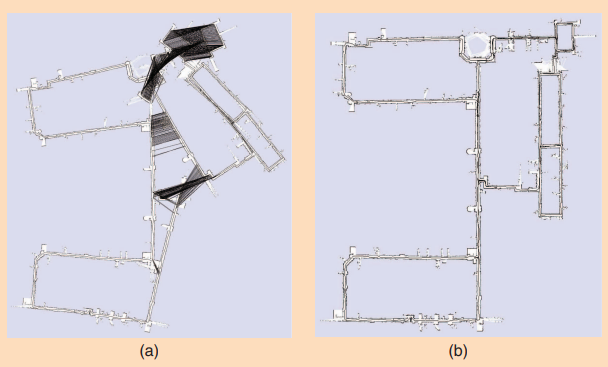
\includegraphics[width=0.4\textwidth]{background/images/slam_graph_optimisation.png}
%       \caption{A diagram showing loop closure and optimisation steps of SLAM pose graph optimisation technique\cite{PoseGraphOptimisation}.}
%       \label{fig:slam_graph_optimisation}
% \end{figure}

% The pose graph optimisation technique relies on memorising the robots relative position and the readings it took in that position. For example we can see a possible robot trajectory in \autoref{fig:slam_diagram}. The robot and its new relative positions are all nodes of the graph and are connected by edges. Whenever a new node is created in the graph, a reading is also taken and stored. Then whenever a new node is visited it is compared with previously stored readings, and if there is a reading that is similar to a very high degree, `loop closure' can take place. In essence this means that the robot is now visiting a location it has already visited, and so the nodes can be joined together. Then once each the loop has been established the graph has to be optimised so that each edge (and therefore node) is at its most likely position relative to the other edges. The way this is done is that each edge of the graph has a relative certainty associated with it, and this certainty dictates how flexible that particular edge is in the optimisation process. Once the loop has been closed the edges are moved such that the overall certainty of the graph is maximised. Once this is complete the readings can be stitched together to form a map of the environment, and the location of the robot within it is very well defined. This process can be seen clearly in \autoref{fig:slam_graph_optimisation}, where in \textbf{(a)} loop closure takes places, and \textbf{(b)} shows the map created after the subsequent optimisation phase. The maps are created using `binary occupancy grids' or `probabilistic grids'. The former simply stores binary 1's and 0's on whether a particular section of the grid is occupied or not. The latter adapts this by having probabilities of occupancy for each section rather than just binary values.

% These SLAM algorithms and localisation algorithms in \Cref{ssec:prob_filters}, however, are classical and have been mostly superseded by deep neural networks in most modern day applications. Furthermore, the algorithm in \Cref{ssec:prob_filters} is only applicable to localising the robot, whereas we want to be able to simultaneously map it's surroundings, for which SLAM  was developed. Both these tasks have now been efficiently solved by neural networks for classical frame-based data, but there is still much ongoing research on how to do the same with spiking data.

\section{Image Reconstruction Algorithms} \label{ssec:image_reconstruction}

Image reconstruction has been implemented for event data building on the direct optimised versions of Convolutional Neural Networks (CNNs). An example of this is the network named `U-net'\cite{UNET} which managed to reconstruct a video using 10M parameters to analyse events from an AER camera protocol. Recent work by Rebecq \textit{et al.} illustrates a novel network architecture that reconstructs a video from a stream of events \cite{spikingToVideo}. These methods are purported to allow the introduction of mainstream computer vision research to event cameras. \Cref{fig:spikes_to_video} shows an example of how converting spiking data to a video stream allows for use of classical computer vision algorithms.

\begin{figure}[htb]
      \centering
      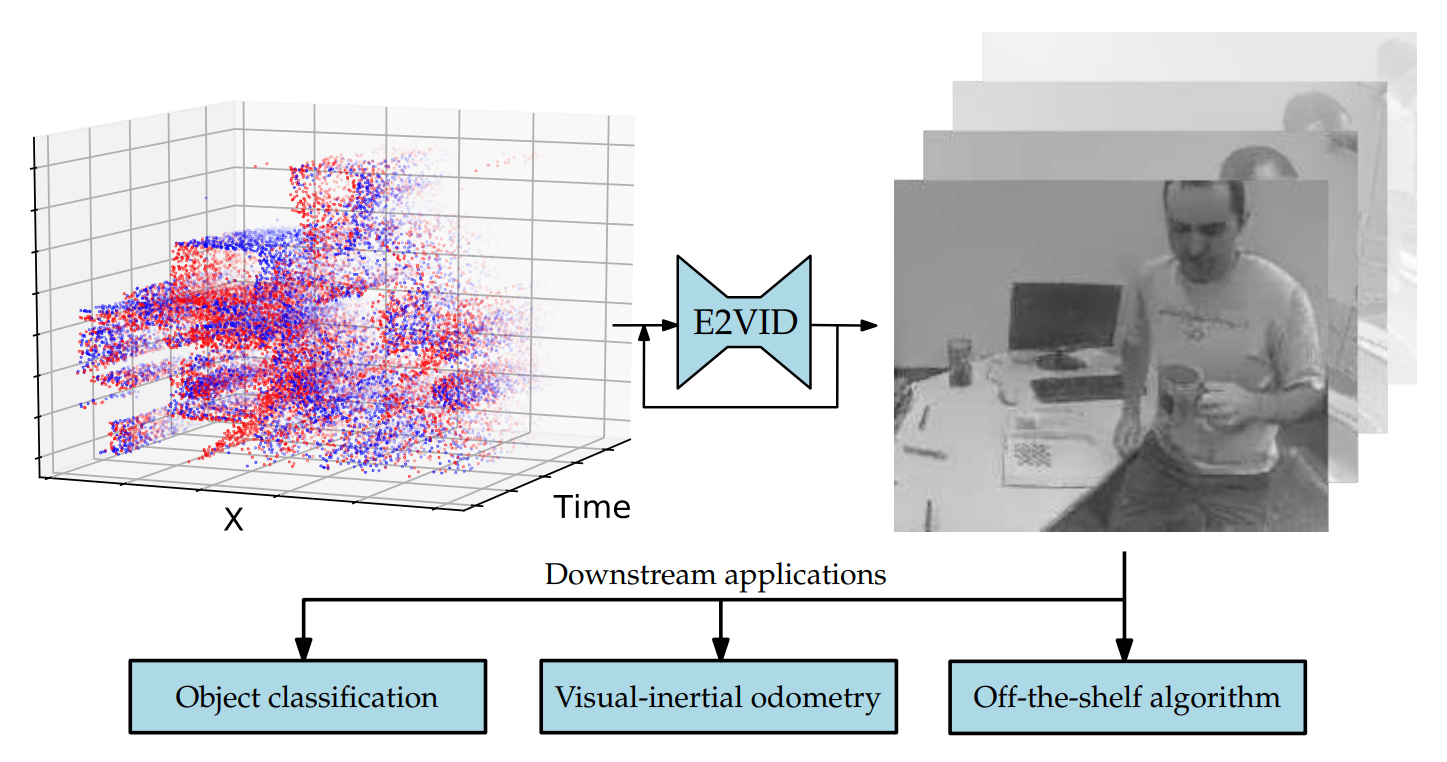
\includegraphics[width=0.7\textwidth]{background/images/spikes_to_video.png}
      \caption{An illustration of the mapping of spiking data to video stream to apply off-the-shelf algorithms to\cite{spikingToVideo}.}
      \label{fig:spikes_to_video}
\end{figure}

A naive approach would be take each event $ e_k = (\boldsymbol{\mathbf{x}}_k, t_l, p_k ) $ and assume that the firing was due to a brightness change above a threshold $ \pm C $ which is a constant that could be set by the user. If this was the case events could be directly integrated to recover the intensity map of images. however, the value $ C $ in reality does not remain constant and is heavily dependent on other factors such as event rate, temperature, and sign of brightness change. The implementation outlined instead makes use of a Recurrent Neural Network (RNN), that takes as input sets of events within a spatio-temporal window. For example, a stream of events will be broken down into sequences given by $ \epsilon_i \: \forall i \in [0, N-1] $. Since each sequence is of fixed length $ N $ the framerate of the output video from the RNN is proportional to the event rate. \Cref{fig:spikes_to_video_rnn} shows the functionality of such a network. Each event window $ \epsilon_k $ is converted to a 3D event tensor and passed into the network along with the last $ K $ constructed images to generate the latest iteration of the image. It is clear from this that each new image is constructed by fusing the previous K images with the new stream of events.

\begin{figure}[htb]
      \centering
      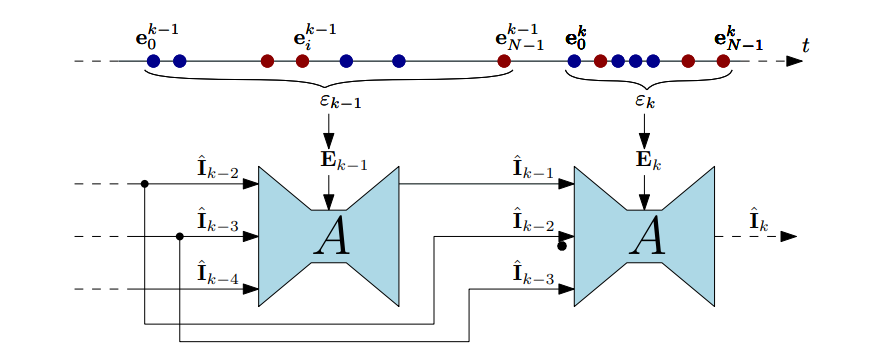
\includegraphics[width=0.6\textwidth]{background/images/spikes_to_video_rnn.png}
      \caption{An overview of RNN used to generate video from sets of events\cite{spikingToVideo}.}
      \label{fig:spikes_to_video_rnn}
\end{figure}

\subsection{Black-box Network}

A method such as the one described in \cref{ssec:image_reconstruction} allows for the use of hugely researched and well documented computer vision algorithms for classification and other tasks while maintaining the benefits of event-based cameras. However, it may be possible to bypass the intermediate step of video reconstruction altogether, and simply create a model that simply acts as a black box and can be trained to give the required output directly from a neuromorphic input. \Cref{fig:temporal_filter} shows how a frame-based video is converted to a continuous stream of events from which snapshots of events can be taken. It should be noted that the distribution of the data from the neuromorphic camera is much more dense than the frame-based video, which means that the motion blue visible in the video should not be a problem with the new representation (as explained in \cref{ssec:event_camera_benefits}).

\begin{figure}[htb]
      \centering
      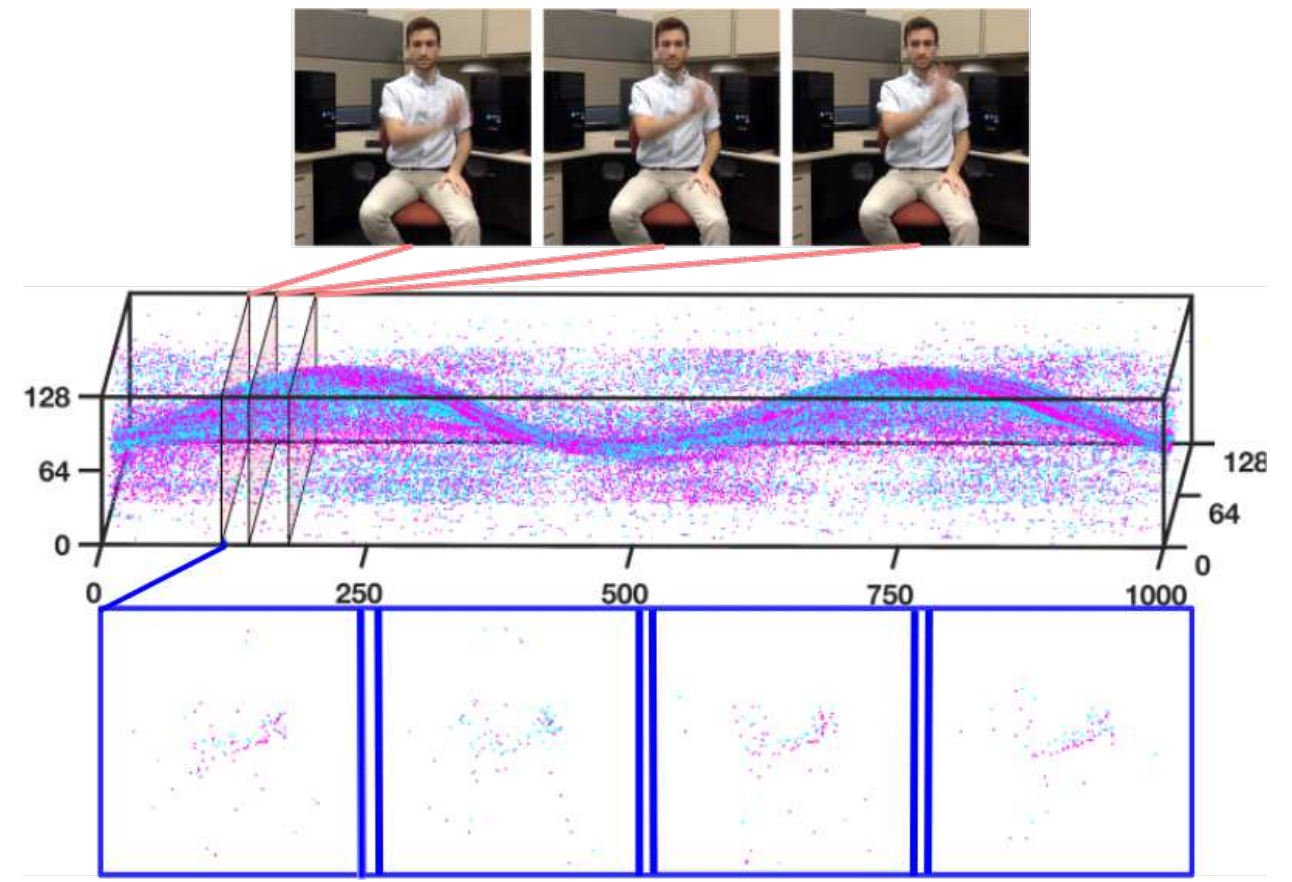
\includegraphics[width=0.6\textwidth]{background/images/temporal_filter.png}
      \caption{An illustration of a temporal filter that caches events fired from a camera\cite{eventBasedGestureRec}.}
      \label{fig:temporal_filter}
\end{figure}

In a paper by Arnon Amir \textit{et al.}\cite{eventBasedGestureRec} a system was created to perform gesture recognition from event-based data. It makes use of the a system such as the one shown in \cref{fig:temporal_filter} to act as one of a set of temporal filters in a cascade. This cascade feeds into a convolution layer and in the end a winner takes all filter is applied to identify the gesture. The whole network can be seen in \cref{fig:event_to_gesture_rec_network}. The intermediate representations of all the layers can also be seen, showing how important features are being identified similar to how they would have been with traditional frame-based inputs.

\begin{figure}[htb]
      \centering
      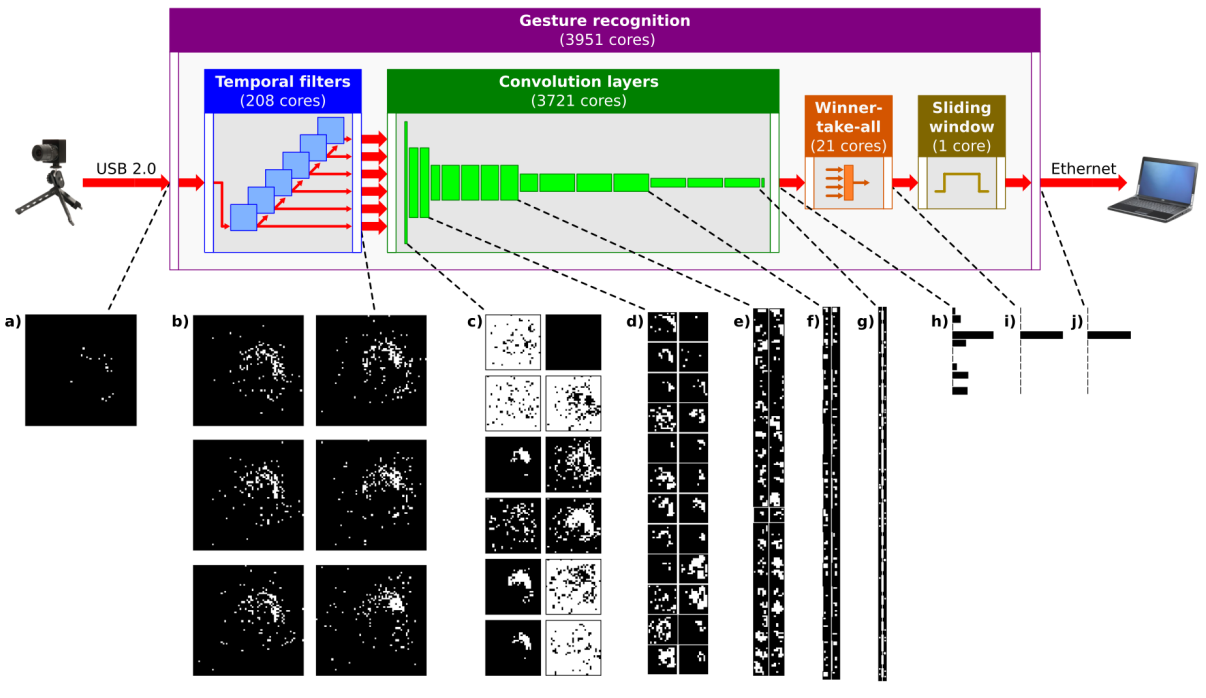
\includegraphics[width=0.6\textwidth]{background/images/event_to_gesture_rec_network.png}
      \caption{A network designed to perform gesture recognition using neuromorphic input by making use of cascading temporal filters\cite{eventBasedGestureRec}.}
      \label{fig:event_to_gesture_rec_network}
\end{figure}

There have been other implementations of systems to carry out complex tasks such as classification, and each has a different way of dealing with spiking input data other than with temporal filters. For example a paper by Xavier Lagorce \textit{et al.}\cite{eventsToTimeSurfaces} moves towards building time surfaces from events to feed into a neural network, whereas Yin Bi \textit{et al.}\cite{eventsToGraphs} propose using a non-uniform sampler to create a graph from events to then feed into a network of so-called graph convolution networks.

\section{Temporally Aware Deep Learning and Classification Models} \label{sec:temporally_aware_models}

\subsection{3-Dimensional Convolutional Neural Network} \label{ssec:3D_conv_network}

Convolutional neural networks have been shown to be much more effective when processing images that networks built solely with dense, fully-connected layers \color{red} TODO: add references here \color{black}. This is because they are able to better identify spacial patterns within an image as a kernel spans more than one pixel. For this reason the basic architecture was to have an input layer (the structure of which is dependent on the input format), followed by a series of hidden convolutional layers of varying parameters.
However, since the input to the system is in fact a 3D tensor of multiple images (i.e. the intensity map video generated from the camera events) a typical convolutional network would not be sufficient to capture the temporal patterns in the data. Typically 2D convolution layers can take as input images with three channels (usually RGB), and so feasibly this coudld be extended to more channels for each frame of the video, but this is not a scalable approach. Instead 3D convolutional layers were used \cite{3DConv}.

\color{red} TODO: Write more about conv3D \color{black}

\subsection{Long-Short Term Memory Networks}

\color{red} TODO: find papers on LSTM \color{black}

\subsection{Gated Recurrent Unit Networks}

\color{red} TODO: find papers on GRU \color{black}

\subsection{Convolutional LTSM Network}

LSTM networks show promise in their ability to find patterns not only on an frame-by-frame basis but also in the time dimension. These spatio-temporal patterns are much more effective for classifying image sequences that just spatial patterns since information is carried throughout the frames to find overall movements and gestures. These LTSMs utilise fully connected layers to find patterns in each frame, however it has been shown that convolutional neural networks produce much better results when operating on image data, and so it would stand to reason that LTSMs would benefit from their structure as well. ConvLSTM, developed by \textit{Xingjian SHI et al.}, showed great promise, and in their experiments captured spatio-temporal correlations better and more consistently FC-LSTM, outperforming it by a sizeable margin in the application of forecasting.

\color{red} TODO: Write more about convLTSM networks etc. \color{black}

\section{Existing Datasets} \label{sec:existing_datasets}

There already exists many repositories of recorded neuromorphic data to get familiar with spiking data. In this section there are some examples of such datasets and a quick overview of their contents.

\subsection{Neuromorphic-MNIST and Other Neuromorphic Datasets} \label{ssec:neuromorphic_datasets}

This dataset is a spiking version of the original frame-based MNIST dataset \cite{MNIST}\cite{NMNIST}. It is identical to the original MNIST dataset, which is a set of handwritten digits, in all ways (including scale, size and sample split) bar one - it was captured using an ATIS sensor mounted on a motorised pan-tilt unit. This sensor moved while viewing the MNIST examples on an external monitor.

For each item in the dataset there is a binary file which has a list of events. Each event is characterised by a 40 bit unsigned integer. The integer gives the following information of a particular event:

\begin{itemize}
      \item bit 39 - 32: X location (in pixels)
      \item bit 31 - 24: Y location (in pixels)
      \item bit 23: Polarity (0 for OFF, 1 for ON)
      \item bit 22 - 0: Timestamp (in microseconds)
\end{itemize}

An example of a visualisation of this data is shown in \cref{fig:nmnist_spikes_visualisation}, where the image used from the MNIST dataset is on the right in part \textbf{(b)} and the resulting spikes from the event-based camera are shown on the left in \textbf{(a)}. Here, `on events' are events where the intensity of a the particular pixel increased by an increment greater than a threshold, and the `off events' are when the intensities decrease by a increment greater than a threshold. The representation is clearly very different to the one given by a classical camera, and therefore the use of such data has to have a different approach to classical techniques.

\begin{figure}[htb]%
      \centering
      \subfloat[\centering]{{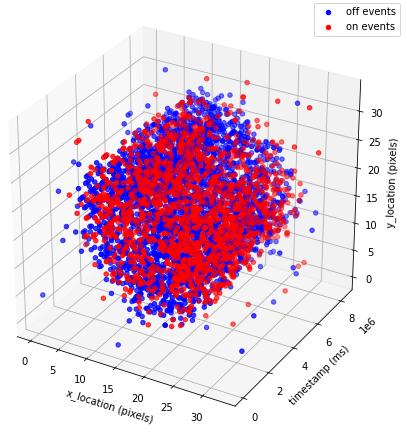
\includegraphics[width=0.35\textwidth]{background/images/nmnist_spikes_visualisation.png}}}%
      \qquad
      \subfloat[\centering]{{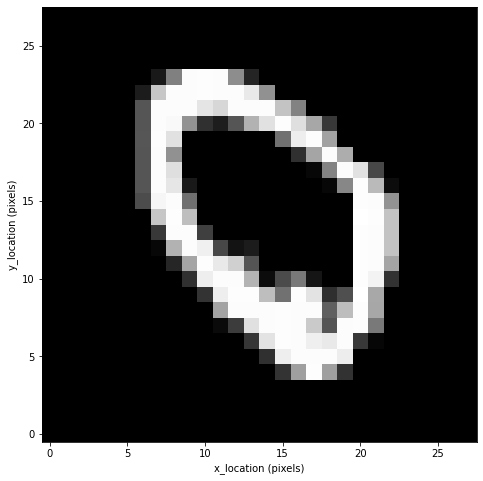
\includegraphics[width=0.35\textwidth]{background/images/mnist_matching_nmnist.png}}}%
      \caption{A visualisation of events from a single training sample from the NMNIST dataset.}%
      \label{fig:nmnist_spikes_visualisation}%
\end{figure}

More examples of neuromorphic datasets include:

\begin{itemize}
      \item \textbf{DVS128}

            This dataset is a set of 11 hand gestures from 29 subjects under 3 illumination conditions. It was created to help create a real-time gesture recognition system that utilises the low power capabilities of event-based cameras\cite{DVS128}.
      \item \textbf{Heridelberg Spiking Datasets}

            The Spiking Heidelberg datasets for spiking neural networks\cite{SpikingHeidelberg} are useful for realising that spiking data is useful for so many more applications than computer vision. This dataset is split into two; The Spiking Heidelberg Digits (SHD) dataset and the Spiking Speech Command (SSC) dataset. Both of these datasets are audio-based classification datasets for which input spikes and output labels are provided.
      
      \item \color{red} \textbf{TODO: Write About The Event-Camera Dataset} \color{black}
\end{itemize}

The above datasets are created using one of a variety of event-based cameras available on the market. the function of each of the cameras is fundamentally similar (as described in \cref{ssec:event_camera_function}) but they also have some differences between them. The cameras widely available today are shown in \cref{fig:camera_models}.

\begin{figure}[htb]
      \centering
      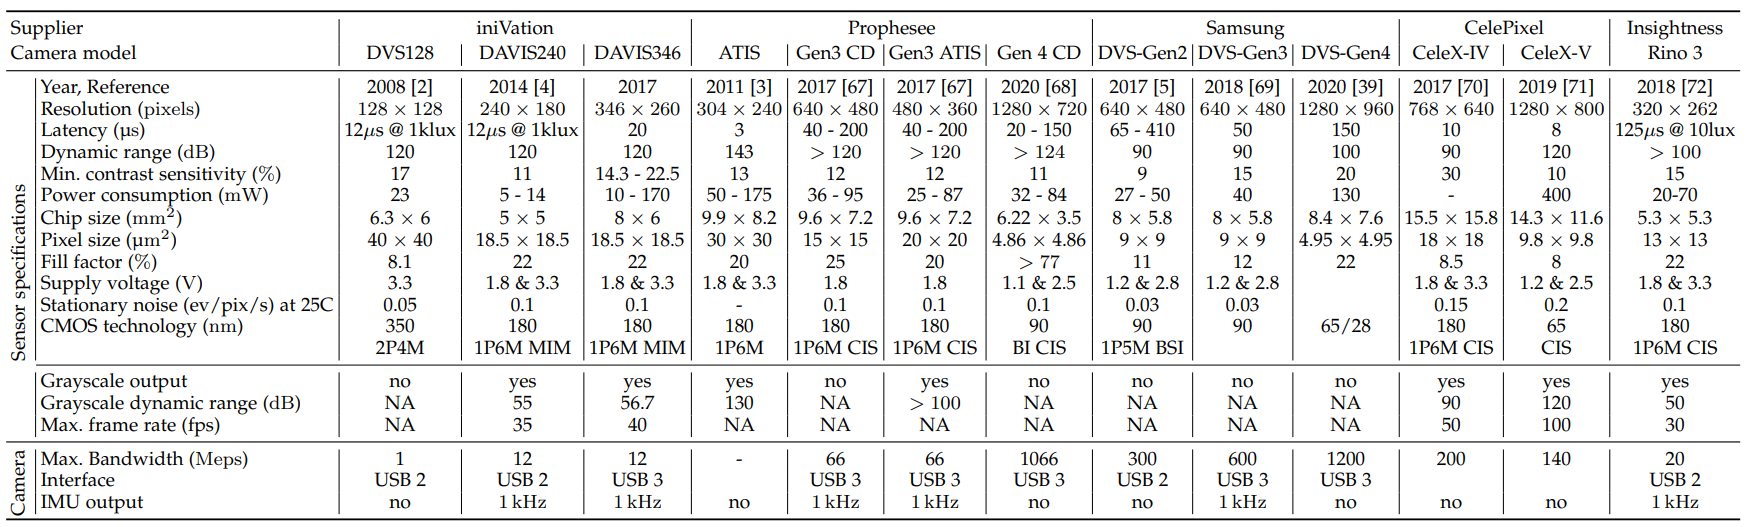
\includegraphics[width=\textwidth]{background/images/camera_models.png}
      \caption{A table listing widely available event-based cameras and their respective features\cite{EventBasedVisionASurvery}.}
      \label{fig:camera_models}
\end{figure}

\subsection{Non-neuromorphic Datasets}

Other data-sets such as fashion-MNIST could also be converted to spiking times by treating image intensities as input currents to model neurons, so that higher intensity pixels would lead to earlier spikes, and lower intensity to later spikes, as was done by Nicolas Perez-Nieves \textit{et al.}\cite{NeuralHetroPromRobLearn}. This avoids having to own an event-based camera to create data (as was done with the NMNIST dataset mentioned in \cref{ssec:neuromorphic_datasets}), which is useful since the cameras are expensive and difficult to get a hold of in general.

\section{Evaluation Metrics} \label{sec:evalutaion_metrics}

The evaluation plan is as given by the typical machine learning pipeline\cite{IntroToML}. \color{red} TODO: Change this to actual used evaluation metrics and check it fits properly in backround \color{black}

For a classification task, when we obtain the results from the test dataset (as shown in \cref{tab:possible_results}) we can calculate a variety of evaluation metrics that give various insights on our final model.

\begin{table}[htb]
    \centering
    \begin{tabular}{|| c  | c ||}
        \hline
        Labels     & Predictions \\
        \hline \hline
        1          & 1           \\
        \hline
        1          & 2           \\
        \hline
        3          & 8           \\
        \hline
        9          & 9           \\
        \hline
        6          & 9           \\
        \hline
        $ \vdots $ & $ \vdots $  \\
    \end{tabular}
    \caption{A table showing an example of results when inputting test data from NMNIST dataset\cite{NMNIST} into the final model.}
    \label{tab:possible_results}
\end{table}

\subsection{Confusion matrix}

Confusion matrices act as a visualisation of a systems performance. It shows possible true labels as well as possible predicted labels on either side, and filled in are the number of results that fit in each segment. In \cref{tab:confusion_matrix} the confusion matrix for the NMNIST dataset is shown as an example. It should be noted that a similar confusion matrix should be created taking each class as positive, then each metric can be calculated by taking the averages (as shown in \cref{ssec:eval_metric_averaging}). For each of the cells the number of matching records are stored to calculate each of the evaluation metrics. The table includes True Positives (TP), False Positives (FP), True Negatives (TN) and False Negatives (FN).

\begin{table}[htb]
    \centering
    \begin{tabular}{|| c c | c | c | c | c ||}
        \hline
                                                                         &                                    & \multicolumn{4}{ c ||}{\textbf{Predicted Class}}                                        \\
        \cline{3-6}
                                                                         &                                    & 1                                                & 2          & 3          & $ \hdots $ \\
        \hline
        \multirow{6}{*}{\rotatebox[origin=c]{90}{\textbf{Actual Class}}} & \multicolumn{1}{| c |}{1}          & TP                                               & FN         & FN         & $ \hdots $ \\
        \cline{2-6}
                                                                         & \multicolumn{1}{| c |}{2}          & FP                                               & TN         & TN         & $ \hdots $ \\
        \cline{2-6}
                                                                         & \multicolumn{1}{| c |}{3}          & FP                                               & TN         & TN         & $ \hdots $ \\
        \cline{2-6}
                                                                         & \multicolumn{1}{| c |}{4}          & FP                                               & TN         & TN         & $ \hdots $ \\
        \cline{2-6}
                                                                         & \multicolumn{1}{| c |}{5}          & FP                                               & TN         & TN         & $ \hdots $ \\
        \cline{2-6}
                                                                         & \multicolumn{1}{| c |}{$ \vdots $} & $ \vdots $                                       & $ \vdots $ & $ \vdots $ & $ \ddots $ \\
    \end{tabular}
    \caption{a table showing one particular confusion matrix for NMNIST dataset\cite{NMNIST} for class 1 as the positive class.}
    \label{tab:confusion_matrix}
\end{table}

\subsection{Accuracy}

The accuracy of the system is the proportion of samples correctly classified.

$$ Accuracy = \frac{TP + TN}{TP + TN + FP + FN} $$

Note: classification error can also be used and is defined as $ 1 - accuracy $.

\subsection{Precision}

Precision is the proportion of positively predicted samples identified correctly.

$$ Precision = \frac{TP}{TP + FP} $$

It should be noted that a high precision may mean that there are many false positives.

\subsection{Recall}

Recall is the proportion of actual positives correctly classified.

$$ Recall = \frac{TP}{TP + FN} $$

It should be noted that a high recall may mean a lot of positive samples may be missed.

\subsection{F-measure/F-score}

This is defined as the harmonic mean of precision and recall in order to get one number as an average measure of performance.

$$ F_1 = \frac{2 \cdot precision \cdot recall}{precision + recall} $$

\subsection{Micro and Macro Averaging} \label{ssec:eval_metric_averaging}

Macro-averaging involves taking an average on the class level. Metrics are calculated for each class and then averaged at the end. Micro-averaging involves taking an average on the item level (i.e., taking the average of each of TP, FP, TN and FN to get the averages metrics).
% \chapter{Implementation Plan}

\section{Timeline}

% oct 22 - jun 6
\begin{figure}[htb]
    \centering
    \begin{ganttchart}[x unit=0.5cm,
            y unit title=0.5cm,
            y unit chart=0.6cm]{1}{18}
        % \gantttitle{Project Timeline}{18} \\
        \gantttitlelist{1,...,18}{1} \\
        \ganttgroup{Inception Report}{1}{2} \\
        \ganttbar{Summary of Deliverables}{1}{1} \\
        \ganttlinkedbar{Background Research Plan}{2}{2} \ganttnewline
        \ganttgroup{Interim Report}{3}{8} \\
        \ganttbar{Project Specification}{3}{3} \\
        \ganttlinkedbar{Background Research}{4}{6} \\
        \ganttlinkedbar{Implementation Plan}{7}{8} \\
        \ganttbar{Evaluation Plan}{7}{8} \\
        \ganttbar{Ethical, Legal, Safety Plan}{7}{8} \\
        \ganttgroup{Final Report}{9}{16} \\
        \ganttbar{Understanding Data}{9}{9} \\
        \ganttlinkedbar{Create Sequantial NN System}{10}{10} \\
        \ganttlinkedbar{Create Parallel NN System}{11}{11} \\
        \ganttmilestone{Classification}{11} \ganttnewline
        \ganttlink{elem12}{elem13}
        \ganttbar{Set-up Camera}{12}{12} \\
        \ganttlinkedbar{Test System on Camera Data}{13}{13} \\
        \ganttmilestone{Experimental Setup}{13} \ganttnewline
        \ganttlink{elem15}{elem16}
        \ganttlinkedbar{Convert System for SLAM}{14}{16} \ganttnewline
        \ganttbar{Evaluate Created Systems}{14}{16}  \\
        \ganttgroup{Final Presentation}{17}{18} \\
        \ganttbar{Prepare Presentation}{17}{18} \\
        \ganttbar{Proof Reading}{17}{18}
    \end{ganttchart}
    \caption{Gantt chart showing fortnightly progress}
    \label{fig:gantt_chart}
\end{figure}

\newpage
\section{Objectives}

\definecolor{Gray}{gray}{0.9}
\newcolumntype{P}[1]{>{\raggedright\let\newline\\\arraybackslash\hspace{0pt}}p{#1}}
% \begin{figure}
\begin{longtable}{|| P{0.2\textwidth} | P{.45\textwidth} | P{.15\textwidth} ||}
    \hline
    \rowcolor{Gray} \multicolumn{1}{|| c}{\textbf{Name}} & \multicolumn{1}{| c |}{\textbf{Description}}                                                                                                                                                                                                                                                                                                                                                                                      & \multicolumn{1}{c ||}{\textbf{Timeline} } \\
    \hline \hline \endhead
    Summary of Deliverables                              & Creating initial plan of deliverables to be present in final project. As well as this it is important to have some initial plans for fall-backs to ensure that a complete project can be achieved.                                                                                                                                                                                                                                & Timeline                                  \\
    \hline
    Background Research Plan                             & Create an initial list of relevant papers to kickstart project.                                                                                                                                                                                                                                                                                                                                                                   & Timeline                                  \\
    \hline
    Project Specification                                & Create a specification that precisely defines the goals of project as well as fall-backs for each case.                                                                                                                                                                                                                                                                                                                           & Timeline                                  \\
    \hline
    Background Research                                  & Use initial list of papers to conduct research behind the topic of the project. This involves looking at previous works and their respective gaps in knowledge. This is in order to give a basis on which to begin implementation, as it should provide all necessary tools and knowledge to begin initial preparations. It is also useful so give an  insight on the need for the project and what problems it aims to overcome. & Timeline                                  \\
    \hline
    Implementation Plan                                  & Using analysis from background reading create a structured implementation plan outlining objectives and milestones, including a deadline for each.                                                                                                                                                                                                                                                                                & Timeline                                  \\
    \hline
    Evaluation Plan                                      & Create a structure for the evaluation of any implemented material, including detailed explanations fo any formula and significance of any values when compared to baselines.                                                                                                                                                                                                                                                      & Timeline                                  \\
    \hline
    Ethical, Legal, Safety Plan                          & Critically evalutate any ethical, legal or safety concerns that many arise as a result of this project and outline various ways in which to mitigate any possible issues.                                                                                                                                                                                                                                                         & Timeline                                  \\
    \hline
    Understanding Data                                   & Load and evaluate the utility of various data-sources and pre-process them ready for use in future NNs.                                                                                                                                                                                                                                                                                                                           & Timeline                                  \\
    \hline
    Create Sequential NN System                          & Create model that first reconstructs frame based video from neuromorphic data to then pass into adaptations of existing networks that carry out classification on frame-based videos.                                                                                                                                                                                                                                             & Timeline                                  \\
    \hline
    Create Parallel NN System                            & Create a single NN that takes neuromorhpic data and directly creates the required output (classification or SLAM).                                                                                                                                                                                                                                                                                                                & Timeline                                  \\
    \hline
    Set-up Camera                                        & Create set-up to obtain real-world data from event-based camera. This also required to create a pipeline to process data to be used in created NNs.                                                                                                                                                                                                                                                                               & Timeline                                  \\
    \hline
    Test System on Camera Data                           & Since real world data may be less idealised than pre-existing datasets, it is important to test the functionality of the system with data obtained from camera. As well as this tests can be done under various more extreme circumstances to test robustness of system.                                                                                                                                                          & Timeline                                  \\
    \hline
    Convert System for SLAM                              & Change function of ststem and train for SLAM rather than classification.                                                                                                                                                                                                                                                                                                                                                          & Timeline                                  \\
    \hline
    Evaluate Created Systems                             & Use metrics listed in the evaltuation plan to check the performance of the system in order to compare each iteration in the project to each other as well as other existing solutions from other researchers.                                                                                                                                                                                                                     & Timeline                                  \\
    \hline
    Prepare Presentation                                 & Create slides and content to present final project results.                                                                                                                                                                                                                                                                                                                                                                       & Timeline                                  \\
    \hline
    Proof Reading                                        & Check through report and presentation to remove errors and make any last-minute changes,                                                                                                                                                                                                                                                                                                                                          & Timeline                                  \\
    \hline
    \caption{Explanations of objectives given in \autoref{fig:gantt_chart}}
    \label{tab:objectives_table}
\end{longtable}
% \chapter{Evaluation Plan} \label{chap:evaluation_plan}

The evaluation plan is as given by the typical machine learning pipeline\cite{IntroToML}. \color{red} TODO: Change this to actual used evaluation metrics \color{black}

\section{Dataset Preparations}

\subsection{Dataset Splitting}

It is commonplace to split the shuffled dataset into  three segments; training, validation and testing. The training data is what is used during each iteration of the back-propagation process. The validation data is what is unseen during this process and is instead used to give an estimation of a models performance while training hyper-parameters. Finally, the testing data is withheld until it is needed to compare different final implementations with each other. It is vital the the training and validation data are withheld while training since otherwise they would not serve as a simulation of unknown data to measure the performance of the system in an unbiased manner. Common splits for training, validation and testing datasets are 60\%/20\%/20\% and 80\%/10\%/10\%  respectively.

\subsection{Dataset Cross-validation}

With smaller datasets the splitting of data may mean that there is too little left to train with. This problem can be alleviated by using cross-validation. This method entails dividing the dataset into a certain number of segments. Then in the first iteration of the learning process, the first segment is used as testing data while the rest is used as training and validation. Then in the next iteration the process can be repeated by using the second segment as the testing, and so on until each segment has been used as testing data. Finally we can use the average of the errors for each testing dataset as the `global error estimate'. It can be noted that the same segmentation and iteration process can be used for the training and validation datasets.

\section{Evaluation Metrics}

For a classification task, when we obtain the results from the test dataset (as shown in \autoref{tab:possible_results}) we can calculate a variety of evaluation metrics that give various insights on our final model.

\begin{table}[htb]
    \centering
    \begin{tabular}{|| c  | c ||}
        \hline
        Labels     & Predictions \\
        \hline \hline
        1          & 1           \\
        \hline
        1          & 2           \\
        \hline
        3          & 8           \\
        \hline
        9          & 9           \\
        \hline
        6          & 9           \\
        \hline
        $ \vdots $ & $ \vdots $  \\
    \end{tabular}
    \caption{A table showing an example of results when inputting test data from NMNIST dataset\cite{NMNIST} into the final model.}
    \label{tab:possible_results}
\end{table}

\subsection{Confusion matrix}

Confusion matrices act as a visualisation of a systems performance. It shows possible true labels as well as possible predicted labels on either side, and filled in are the number of results that fit in each segment. In \autoref{tab:confusion_matrix} the confusion matrix for the NMNIST dataset is shown as an example. It should be noted that a similar confusion matrix should be created taking each class as positive, then each metric can be calculated by taking the averages (as shown in \Cref{ssec:eval_metric_averaging}). For each of the cells the number of matching records are stored to calculate each of the evaluation metrics. The table includes True Positives (TP), False Positives (FP), True Negatives (TN) and False Negatives (FN).

\begin{table}[htb]
    \centering
    \begin{tabular}{|| c c | c | c | c | c ||}
        \hline
                                                                         &                                    & \multicolumn{4}{ c ||}{\textbf{Predicted Class}}                                        \\
        \cline{3-6}
                                                                         &                                    & 1                                                & 2          & 3          & $ \hdots $ \\
        \hline
        \multirow{6}{*}{\rotatebox[origin=c]{90}{\textbf{Actual Class}}} & \multicolumn{1}{| c |}{1}          & TP                                               & FN         & FN         & $ \hdots $ \\
        \cline{2-6}
                                                                         & \multicolumn{1}{| c |}{2}          & FP                                               & TN         & TN         & $ \hdots $ \\
        \cline{2-6}
                                                                         & \multicolumn{1}{| c |}{3}          & FP                                               & TN         & TN         & $ \hdots $ \\
        \cline{2-6}
                                                                         & \multicolumn{1}{| c |}{4}          & FP                                               & TN         & TN         & $ \hdots $ \\
        \cline{2-6}
                                                                         & \multicolumn{1}{| c |}{5}          & FP                                               & TN         & TN         & $ \hdots $ \\
        \cline{2-6}
                                                                         & \multicolumn{1}{| c |}{$ \vdots $} & $ \vdots $                                       & $ \vdots $ & $ \vdots $ & $ \ddots $ \\
    \end{tabular}
    \caption{a table showing one particular confusion matrix for NMNIST dataset\cite{NMNIST} for class 1 as the positive class.}
    \label{tab:confusion_matrix}
\end{table}

\subsection{Accuracy}

The accuracy of the system is the proportion of samples correctly classified.

$$ Accuracy = \frac{TP + TN}{TP + TN + FP + FN} $$

Note: classification error can also be used and is defined as $ 1 - accuracy $.

\subsection{Precision}

Precision is the proportion of positively predicted samples identified correctly.

$$ Precision = \frac{TP}{TP + FP} $$

It should be noted that a high precision may mean that there are many false positives.

\subsection{Recall}

Recall is the proportion of actual positives correctly classified.

$$ Recall = \frac{TP}{TP + FN} $$

It should be noted that a high recall may mean a lot of positive samples may be missed.

\subsection{F-measure/F-score}

This is defined as the harmonic mean of precision and recall in order to get one number as an average measure of performance.

$$ F_1 = \frac{2 \cdot precision \cdot recall}{precision + recall} $$

\subsection{Micro and Macro Averaging} \label{ssec:eval_metric_averaging}

Macro-averaging involves taking an average on the class level. Metrics are calculated for each class and then averaged at the end. Micro-averaging involves taking an average on the item level (i.e., taking the average of each of TP, FP, TN and FN to get the averages metrics).

\section{Baselines for Comparison}

In order to measure the performance of the system against current solutions it is useful to have a list of baseline performances. This way it can be inferred if there is an improvement being made by any newly created systems. Examples of systems that can be used include the reconstruction algorithm posed by H. Rebecq \textit{et al.}\cite{spikingToVideo} and existing gesture recognition algorithms for the DVS128 dataset\cite{DVS128} like the one posed by Arnon Amir \textit{et al.}\cite{eventBasedGestureRec} (See both in \Cref{sec:existing_algorithms}).

\section{Additional Testing with Camera}

If the model were to train using only the datasets available, there is a risk that the data would be unbalanced and the network is training on a very specific set of idealised readings. Testing with extraneous data generated by a camera under various different conditions would allow for evaluating the performance of the networks on data that is completely unseen and dissimilar.
% \chapter{Ethical, Legal and Safety Plan} \label{chap:ethical_plan}

In general the project in unproblematic, and poses minimal safety risks other than the ones presented when working with computers for extended periods of time (e.g., RSI, eye-strain, back aches etc.). In terms of ethical and legal considerations, however, it is important to make sure to use the practical camera setup in a sound manner. When collecting data from others it is important to be mindful of privacy issues. Consent must be taken from any participants if ever the need arises to take videos of others, but for the vast majority of project only videos of myself will be taken. As well as this it is important to consider where the system may be used if it is every put into production. Especially in IoT applications, privacy is of utmost concern, luckily with spiking data, if an intermediate video reconstruction cannot be obtained from the system, very little information can be discerned from spiking data. Therefore it would be very difficult to identify any individual within neuromorphic data itself.
\chapter{Analysis and Design} \label{chap:analysis_and_design}

This chapter outlines overall design for the project as well as the analysis that formed the basis of each decision. The design of the project is mostly guided by the requirements set out in \cref{chap:introduction}. Building on the work described in \cref{chap:background}, novel pipelines are designed to advance the field of neuromorphic processing. The choice of programming language and other software/hardware tools, the processing of each dataset, and finally the structure of various classification pipelines are all set out before the implementation part of the report. As well as this a new frame-integration method is proposed, as well as state-of-the-art classification networks. The final part of this chapter also creates a framework for the comparison of each network, which can be found in \cref{chap:testing_and_results}.

\section{Hardware and Software}

\subsection{Programming Languages}

When choosing a programming language for the project there were a few choices that are most often chosen by developers; Python\cite{Python}, R\cite{R}, and C++\cite{C++}. Python is the most popular choice due to the ease with which algorithms can be developed using it. Python features an extensive list of libraries and debugging functions that are invaluable when creating machine learning algorithms in particular, making the language of choice for this project. It is also important to note, however, the benefits of the other language options. C++ often results in programs with impressive performance due to the ability it grants to make low-level processes more efficient. Unfortunately this fine-level control also opens up programmers to more a demanding and time-intensive programming experience, with much more code writing and debugging to be done manually. R would also be a great choice for machine learning, and shares many similarities with Python, being open-source and having a huge community of developers constantly building libraries and tools. It has a different approach to machine learning, with a a more statistical analysis emphasis. Therefore Python remains the best choice for a more general approach for data processing.

\subsection{Machine Learning Frameworks and Software}

\subsubsection{PyTorch}

Pytorch\cite{Pytorch} is a relatively new framework for machine learning, and provides a developer friendly way to write machine learning code. It has a more `pythonic' approach to code abstraction than its competition in the space, and the \emph{torch.nn.module} gives access to clear, reusable module definitions in an Object-Oriented Programming (OOP) manner. It also allows for simple data parallelism, so that batch processing can easily be split over different sets of hardware. It also has an intuitive debugging experience since it can use standard debugging tools such as PyCharm and pdb.

\subsubsection{Tensorflow}

Tensorflow\cite{Tensorflow} is the older and more widely adopted machine learning library. It provides a more robust set of functionality with clear documentation. In terms of deployment it is the clear favourite as it allows models to be deployed on specialised servers and even on mobile. When visualising data software such as TensorBoard are ideal as it includes functionality to display model graphs, variables, histograms and much more. As well as this, Keras\cite{Keras} is a framework developed by Google, and uses a primarily Tensorflow based back-end. It provides an easy to use API for fast prototyping and high levels of abstraction. It is used commercially by a plethora of companies and has a vast and highly developed research community. For these reasons Keras using a Tensorflow back-end were chosen for this project.

\subsection{Other Software}

\subsubsection{SpikingJelly}

SpikingJelly\cite{SpikingJelly} is an open-source deep learning framework for Spiking Neural Network (SNN) based on PyTorch. It allows for the processing of many often-used datasets in the neuromorphic community (Some of which are described in \cref{sec:existing_datasets}), as well as a simple set of classes for building SNNs or converting ANNs to SNNs. The library, which was mainly co-developed by the Multimedia Learning Group, the Institute of Digital Media (NELVT), the Peking University and Peng Cheng Laboratory, can be installed directly via the \emph{pip} command. Using it, data can be loaded as event streams, as well as integrated frames (described in \cref{ssec:frame_integration}) of varying frame lengths or frame-rates. As well as this the package features clear documentation and tutorials to begin analysing neuromorphic data.

\subsubsection{NengoDL} \label{sssec:nengo}

NengoDL\cite{NengoDL} is a software framework designed to combine the strengths of neuromorphic modelling and deep learning. It is a useful tool for constructing biologically inspired spiking neuron models, and combining them to create fully spiking neural networks. As well as this, these networks are intermixed with efficiently simulated deep learning concepts such as convolutional neural networks. This unified framework therefore allows us to train SNNs in the same way as we would for other ANN models with an easy to use interface. As well as this converters exist in order to convert ANNs to SNNs with relative ease.

\subsection{Cloud Environments}

Since Python is the language of choice for the project, Python Notebooks are a good choice for code segmentation and presentation. They allow for python code to be written in executable cells, so that their output, as well as other text, can be presented in a full document. This makes the code easy to understand for others, and good for development as well. Python notebooks can be run locally on a web server, as well as online on a cloud service. Many machine learning frameworks and algorithms make use of hardware acceleration using GPUs or TPUs. This allows for running code much faster on more powerful machines with this specialised hardware in them. This calibre of hardware was not readily available during the course of the project, so cloud services provided by the likes of Google and Amazon Web Services were used as a good alternative. They allow for the renting of GPUs etc. from their own servers, so that code can be run on them via their respective web services. 

The two main web services available at this time are Google Colaboratory\cite{GoogleColab} and AWS Sagemaker Studio Lab\cite{AwsSagemaker}. In terms of hardware, both services offer access to powerful GPUs, though sagemaker offers the more powerful T4 GPU at the free tier. This benefit, however, is not entirely relevant as a pro subscription would be necessary with either service to make use high-RAM runtimes. Due to Colaboratory's better share-ability and wider adoption, it was chosen as the service for this project.

\section{Datasets}

The datasets used for the evaluation of the networks in this project were NMNIST (\Cref{sssec:nmnist}), DVS128 Gesture (\Cref{sssec:dvs128_gesture}) and CIFAR10-DVS (\Cref{sssec:cifar10_dvs}), since these are the most suited for training on classification tasks. As well as this their recording conditions and topics are varied, meaning an evaluation of the system can be more robust and reliable. The Event Camera Dataset for SLAM (\Cref{sssec:event_camera_dataset}) is also extensive and includes side by side frames from a traditional camera, making it ideal for testing the intensity reconstruction algorithm used in the two-phase pipeline described later in this chapter.

\subsection{Data Pre-processing} \label{ssec:data_preprocessing_design}

Before processing data, z-score standardisation needs to take place. \Cref{eq:z_score} shows the equation dictating the process. In practical terms the standard deviation of $ x $ can be substituted by the max value of $ x $. The reason this needs to occur is to `center' the data, meaning the inputs to the network can be guaranteed to be of a certain scale. In the training process the weights and biases (as described in \cref{eq:artificial_neuron_output}) are applied to the initial inputs, which are then back-propagated based on the loss gradient. The standardisation process ensures that these gradients don't spike out of proportion, meaning the same global learning rate can be used for the network. As well as this parameters are often shared across deep learning networks, and if inputs weren't of a similar scale for every part of an image, for example, then this sharing of parameters wouldn't work since some areas would have a much larger weight than others. It is also important to note that the standard deviation and mean statistics used in this standardisation is always from the training dataset, since it is important to never use values from the testing set since that would invalidate it as a true indication of the network's performance.

\begin{equation}
    x_{scaled} = \frac{x - mean_x}{std_x}
    \label{eq:z_score}
\end{equation}

\section{Two-phase Intensity Reconstruction Models}

In order to make use of existing highly-tested and documented computer vision techniques, an intensity reconstruction of event streams was necessary. For this reason a two-phase network (shown in \cref{fig:two_phase_network_pipeline}) was devised, wherein events are reconstructed into intensity videos before being passed into various classification networks. Each event stream was passed into the E2VID reconstruction network\cite{spikingToVideo}, allowing for each classifier that the data is fed into to analyse more complex visual patterns than were available from the frame-integrated event streams. The rationale behind this is that commonly used neural networks for video analysis are built to detect features from intensity frames rather than event streams. Therefore in order to make use of these specialisations, each event stream needs to be converted into a more common input form.

\begin{figure}[htb]
    \centering
    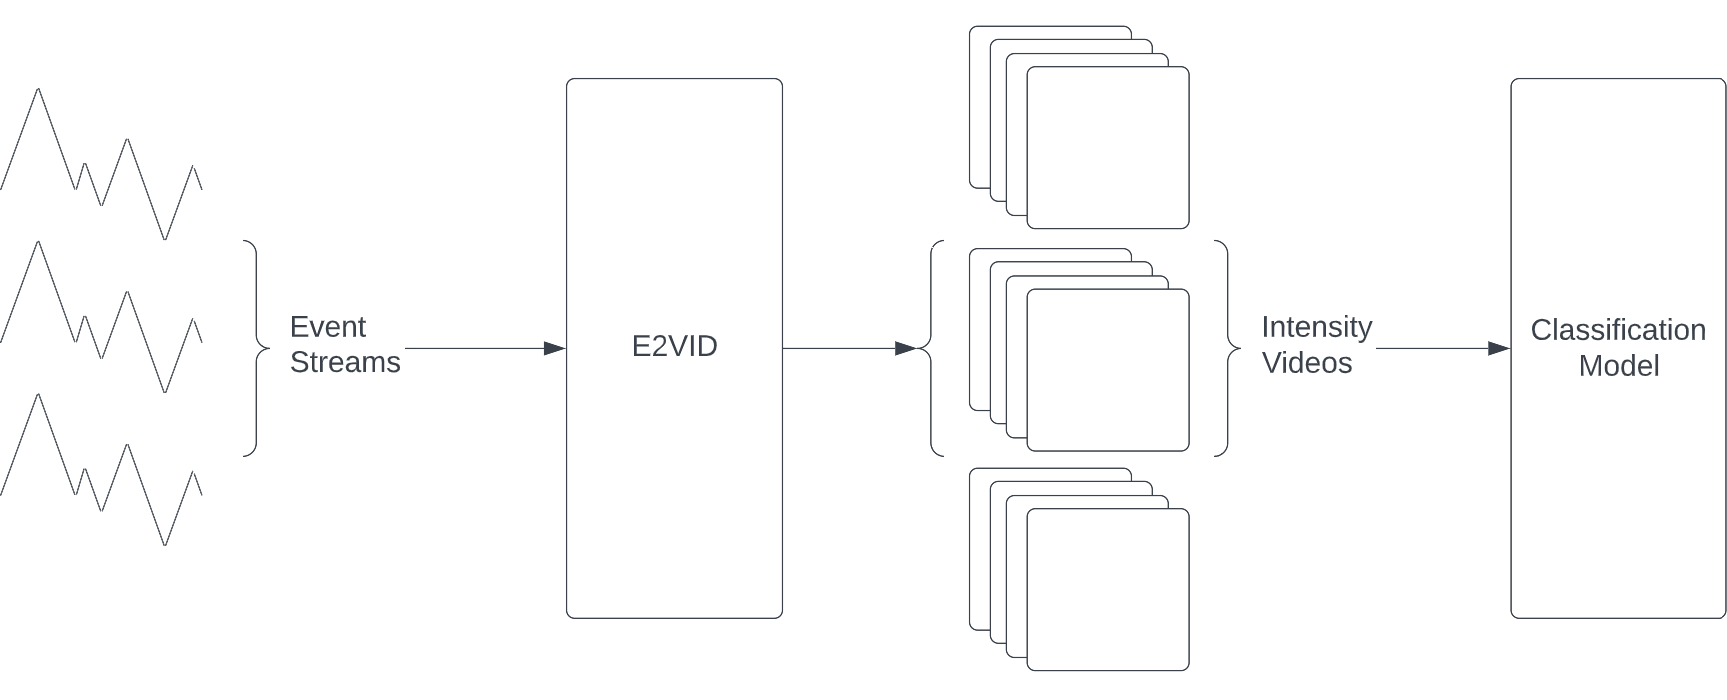
\includegraphics[width=0.85\textwidth]{analysisanddesign/images/two_phase_network_pipeline.png}
    \caption{An illustration of the two-phase classification pipeline.}
    \label{fig:two_phase_network_pipeline}
\end{figure}

\section{End-to-end Event Classification Models} \label{sec:end_to_end_classification_design}

For classifying frames directly, a frame integration method was utilised as described in \cref{ssec:frame_integration}. The method described involves having two channels per created frame. Each channel stores whether a positive or negative event was fired at any one pixel during a given time-slice. There are two variations of time-slice generation, which will be referred henceforth as `synchronous' and `asynchronous' frame-integration. Synchronous frame-integration is named due to the fact that each frame stores event information of a fixed time-frame. For example, each frame could store information for a 10ms time-slice. This means the generated frames are more akin to the outputs of frame-based cameras that have a fixed frame-rate. Asynchronous frame-integration, on the other hand, involves collecting a set number of events for each frame. The benefit of this method is that the amount of information per frame is constant, irrespective of when more or less motion occurs in the video. Another asynchronous approach is to simply divide the events into a set number of segments. Then each segment can be integrated individually. These methods mean that certain frames may encode information over a longer time-span than other frames.

A slight adaptation of the classical method was also devised, in which rather than having binary information of on/off events per pixel of the frame, we could instead have a single channel value for each pixel with the sum of all event polarities for that location. This way the magnitude (or number) of events for each pixel over the time segment can also be captured. A diagram showing the basics of the custom integration process is shown in \cref{fig:frame_integration_diagram}.

For classical frame integration the synchronous frame integration method was used, whereas for custom integration the second asynchronous method was used. Both these methods allow for the number of frames per sample to be constant, making it easier to input into neural networks.

\begin{figure}[htb]
    \centering
    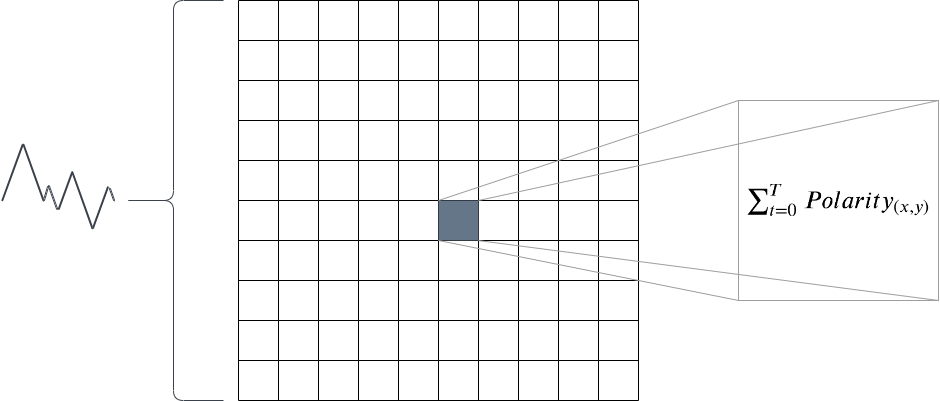
\includegraphics[width=0.8\textwidth]{analysisanddesign/images/frame_integration_illustration.png}
    \caption{An illustration of the frame integration process with custom integrating method.}
    \label{fig:frame_integration_diagram}
\end{figure}

\section{Classification Networks}

Given below are the various networks used to classify either integrated frames or image reconstructions. Each network has its benefits and drawbacks, but there are a few commonalities between them. 

During the training process of each of the networks a callback function was used called\\ \lstinline{EarlyStopping}. This built-in Keras callback allows for the interrupting of network training when the validation accuracy of the network stagnates or falls. This should, in theory, prevent over-fitting to the training data. A patience value is set so that even if accuracy drops for only one epoch it is given the opportunity to rise again. This, of course, means that the training dataset needs to be split into training and validation, where the validation set is more unseen data to evaluate the performance of the networks every epoch. Finally, the most optimal weights are loaded back when the network finishes training. 

As well as this, dropout (or recurrent dropout for LSTM and GRU cases) layers were used. These layers mean that during the training process certain neurons will be `turned off' and therefore not part of the back-propagation process. This should allow the resulting network to be robust since there is no over-reliance on any one neuron of the network.

Finally, for the learning rates for each system, it is necessary to find the optimal value. If the rate is too high, the model will quickly back-propagate to the optimal value, however once it gets close to it the weights may oscillate. This is because only a small step may be needed to make it to the ideal values, but the model constantly overshoots it. On the other hand, if the learning rate is too low, then the learning process will be very slow, and reaching an optimal value may take many epochs. As well as this, for more complex functions the network may get stuck on a local minimum value for the loss. It is clear in this case that an adaptive learning rate would be the most ideal. One would like the rate to be high to start off with, and become smaller and smaller as the training process goes on. This can be done with a Keras callback function, however for the models in this project the Adam optimiser\cite{Adam} was chosen instead. This optimiser implements a function to find the best value for the learning rate itself.

\subsection{3-Dimensional Convolutional Neural Network} \label{ssec:conv_3d_network_design}

A 3D convolutional network, as described in \cref{ssec:3D_conv_network}, was implemented to work on the event data. A diagram showing the function of one of the 3D convolutional layers used in the final network can be seen in \cref{fig:conv3d_diagram}. As opposed to their two dimensional counterparts, 3D convolutions involve taking video streams as input and output, allowing the network to decode patterns in both the spacial and temporal dimensions. As well as this the network employs batch normalisation layers in order to accelerate training. The reason the training time is reduced is that there is some regularisation, meaning the data is rescaled so that it centres around 0 and has a standard deviation of 1. In essence this means the outputs of each intermediate layer look similar in distribution, so the same learning rate can be used for back-propagation throughout the network.

\begin{figure}[htb]
    \centering
    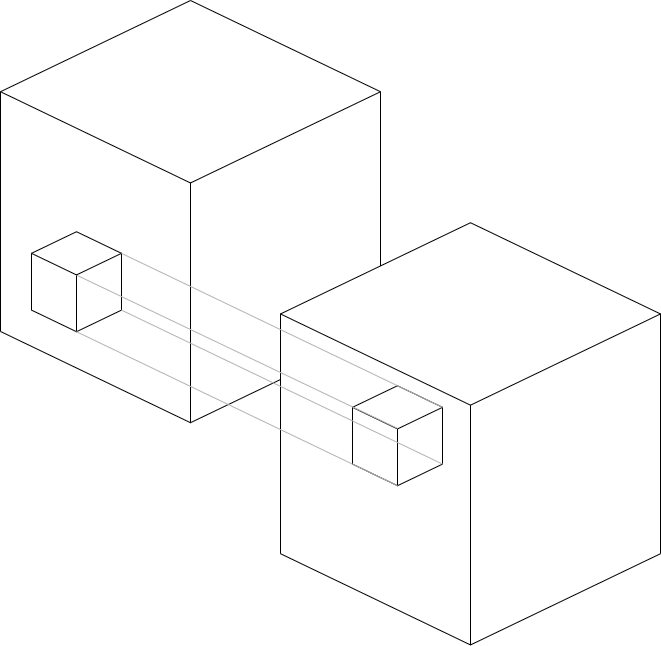
\includegraphics[width=0.4\textwidth]{analysisanddesign/images/conv3d_diagram.png}
    \caption{An illustration of a 3D convolutional layer.}
    \label{fig:conv3d_diagram}
\end{figure}

\subsection{Convolutional LSTM Network}

A convolutional LSTM network as described in \cref{ssec:conv_lstm} was implemented to work on the event data. In this network the video that is fed in is passed through the network one frame at a time. The ConvLSTM layers apply 2D convolution on the frames to extract spacial patterns, and then these features are passed into LSTMs. The LSTMs allow for the network to remember previous frames and therefore analyse temporal features of the data as well.

\subsection{Custom Convolutional LSTM Network}

This network is an extension of the LSTM network in the previous section, adding more capacity for the model to learn spatio-temporal patterns. It involves altering the intermediate convolutional neural network that analyses each frame in the video time series. A diagram showing the pipeline of the overall network can be seen in \cref{fig:custom_conv_lstm_pipeline}. This additional capacity is helpful for deciphering more complex `actions' in a video, such as in the case of gesture recognition.

\begin{figure}[htb]
    \centering
    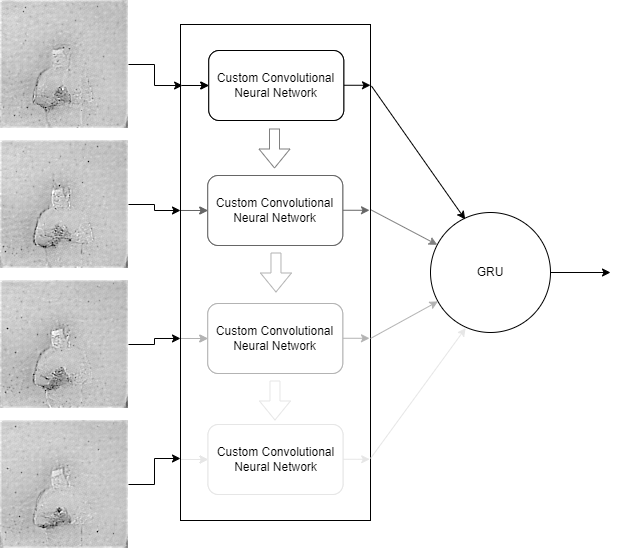
\includegraphics[width=0.65\textwidth]{analysisanddesign/images/custom_conv_lstm_pipeline.png}
    \caption{An illustration of the custom convolutional LSTM network.}
    \label{fig:custom_conv_lstm_pipeline}
\end{figure}

\subsection{Spiking Neural Network} \label{ssec:snn_design}

With this network the whole system, from data generation to classification, could be fully neuromorphic. Using techniques as described in \cref{ssec:snn_and_heterogeneity}, traditional ANNs could easily be converted to SNNs\cite{Ann2Snn} for classification. For the conversion process the \lstinline{nengo_dl} package can be used (see \cref{sssec:nengo}). In order to train the network a differentiable approximation of the spiking neurons was used. This meant that the data could be trained using back-propagation as normal. During inference, however, the actual spiking neurons could be used\cite{TrainingSnn}. Since the network is trained before the conversion from ANN to SNN, the performance of the SNN will not be comparable to the ANN due to approximation errors. These approximations can be improved by changing certain properties of the SNN and checking the performance of the inference.

Spiking neural networks work similarly to ANNs, however there are some key differences. One major difference is in the activation of the neurons. Whereas with non-spiking artificial neurons the output is a continuous function based on the instantaneous input, spiking neurons accumulate inputs and build up to an eventual spike. This means that inputs to the neuron have to be sustained (repeated) for a certain amount of time to allow for this build-up of potential. For our network, since it is a 3D vector of frames over time, the input to the network needs to be a 4D vector. An illustration of the creation of the 3D vectors that were input into the ANN and the subsequent 4D network fed into the spiking equivalent are shown in \cref{fig:sustained_video}.

\begin{figure}[htb]
    \centering
    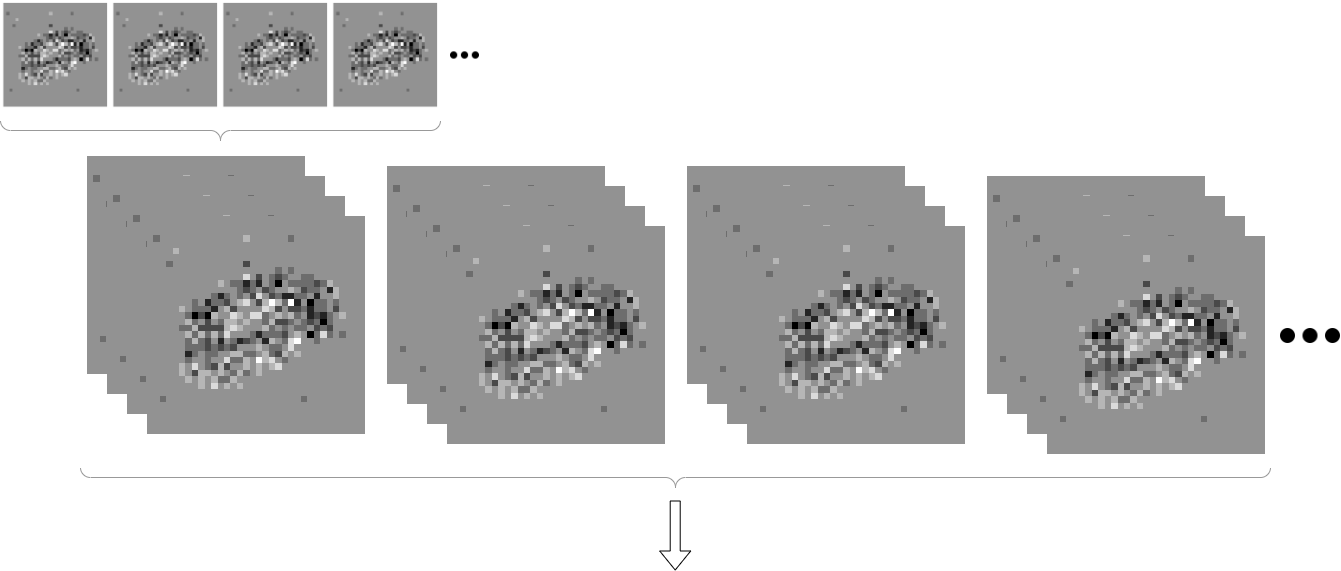
\includegraphics[width=0.75\textwidth]{analysisanddesign/images/sustained_video.png}
    \caption{An illustration of how frames of a video can be repeated for input to a spiking neural network.}
    \label{fig:sustained_video}
\end{figure}

However, unlike convolutional network layers, recurrent layers such as LSTM and GRU do not have a direct conversion available to spiking networks. There is, however, a component known as Legendre Memory Unit (LMU) that are much better suited to the conversion process. Like LSTMs, LMUs have been shown to perform well in a variety of tasks with relatively few internal parameters\cite{LMU}. This unit shows promise for creating more complex networks to analyse time-series data.

\section{Evaluation Metrics} \label{sec:evalutaion_metrics}

The evaluation plan is as given by the typical machine learning pipeline\cite{IntroToML}. For a classification task, when we obtain the results from the test dataset (an example of which is shown in \cref{tab:possible_results}) we can calculate a variety of evaluation metrics that give various insights on our final model.

\begin{table}[htb]
    \centering
    \begin{tabular}{|| c  | c ||}
        \hline
        Labels     & Predictions \\
        \hline \hline
        1          & 1           \\
        \hline
        1          & 2           \\
        \hline
        3          & 8           \\
        \hline
        9          & 9           \\
        \hline
        6          & 9           \\
        \hline
        $ \vdots $ & $ \vdots $  \\
    \end{tabular}
    \caption{A table showing an example of results when inputting test data from NMNIST dataset\cite{NMNIST} into the final model.}
    \label{tab:possible_results}
\end{table}

\subsection{Confusion matrix}

Confusion matrices act as a visualisation of a systems performance. It shows possible true labels as well as possible predicted labels on either side, and filled in are the number of results that fit in each segment. In \cref{tab:confusion_matrix} the confusion matrix for the NMNIST dataset is shown as an example. This type of table is created for each class including the True Positives (TP), False Positives (FP), True Negatives (TN) and False Negatives (FN).

\begin{table}[htb]
    \centering
    \begin{tabular}{|| c c | c | c | c | c ||}
        \hline
                                                                         &                                    & \multicolumn{4}{ c ||}{\textbf{Predicted Class}}                                        \\
        \cline{3-6}
                                                                         &                                    & 1                                                & 2          & 3          & $ \hdots $ \\
        \hline
        \multirow{6}{*}{\rotatebox[origin=c]{90}{\textbf{Actual Class}}} & \multicolumn{1}{| c |}{1}          & TP                                               & FN         & FN         & $ \hdots $ \\
        \cline{2-6}
                                                                         & \multicolumn{1}{| c |}{2}          & FP                                               & TN         & TN         & $ \hdots $ \\
        \cline{2-6}
                                                                         & \multicolumn{1}{| c |}{3}          & FP                                               & TN         & TN         & $ \hdots $ \\
        \cline{2-6}
                                                                         & \multicolumn{1}{| c |}{4}          & FP                                               & TN         & TN         & $ \hdots $ \\
        \cline{2-6}
                                                                         & \multicolumn{1}{| c |}{5}          & FP                                               & TN         & TN         & $ \hdots $ \\
        \cline{2-6}
                                                                         & \multicolumn{1}{| c |}{$ \vdots $} & $ \vdots $                                       & $ \vdots $ & $ \vdots $ & $ \ddots $ \\
    \end{tabular}
    \caption{a table showing one particular confusion matrix for NMNIST dataset\cite{NMNIST} for class 1 as the positive class.}
    \label{tab:confusion_matrix}
\end{table}

\subsection{Accuracy}

The accuracy of the system is the proportion of samples correctly classified.

$$ Accuracy = \frac{TP + TN}{TP + TN + FP + FN} $$

Note: classification error can also be used and is defined as $ 1 - accuracy $.

\subsection{Precision}

Precision is the proportion of positively predicted samples identified correctly.

$$ Precision = \frac{TP}{TP + FP} $$

It should be noted that a high precision may mean that there are many false positives.

\subsection{Recall}

Recall is the proportion of actual positives correctly classified.

$$ Recall = \frac{TP}{TP + FN} $$

It should be noted that a high recall may mean a lot of positive samples may be missed.

\subsection{F-measure/F-score}

This is defined as the harmonic mean of precision and recall in order to get one number as an average measure of performance.

$$ F_1 = \frac{2 \cdot precision \cdot recall}{precision + recall} $$
\chapter{Implementation} \label{chap:implementation}

% - Image Reconstruction
% 	- Reconstruction algorithm (E2VID and data pre-processing etc.)
% 	- Computer vision techniques and models
% 		- NMNIST Classification
% 		- DVS128 Gesture Classification

% - Direct Event Classification
% 	- Data pre-processing etc. (talk briefly about working directly with events with nlp-like method)
% 	- Various model architectures
% 		- NMNIST Classification
% 		- DVS128 Gesture Classification

% - Converting previous networks to SNNs

\section{Two-phase Intensity Reconstruction Models}

The models described above allow for the system to learn directly on the spiking data. Another approach that was taken was to attempt to utilise video reconstruction networks to the event data so that more classical models and architectures could be used to patterns in the data.

\subsection{Reconstruction Algorithms}

\subsubsection{E2VID}

E2VID, as described in \color{red} TODO: Reference background reading here \color{black}, is a state-of the art network based on UNET that reconstructs intensity videos from events data. Having gotten the output from the network (which on test data had 90\% accuracy \color{red} TODO: check accuracy figure \color{black})

\color{red} TODO: all of the following;

\begin{itemize}
    \item Similar to denoising network CNN more easily able to find patterns in data
    \item gesture intensity maps equivalent to 100fps but retains high frequency information without too much noise
    \item spikingjelly for integrating frames which is widely used approach
\end{itemize}

\color{black}

\subsection{Classification Models on Reconstructed Video Output}

\section{End-to-end Event Classification Models}

\subsection{Data Preprocessing}

A common method of processing events streams to get integrated frames is given in \cref{ssec:frame_integration}. This technique was applied to three readily available data-sets; NMNIST, DVS128 Gesture and CIFAR10-DVS.

\begin{figure}[htb]%
    \centering
    \subfloat[\centering]{{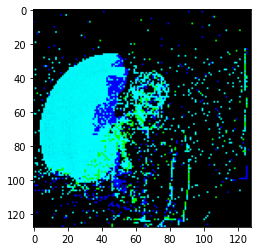
\includegraphics[width=0.25\textwidth]{implementation/images/Dvs128_integrated_frame_1.png}}}%
    \qquad
    \subfloat[\centering]{{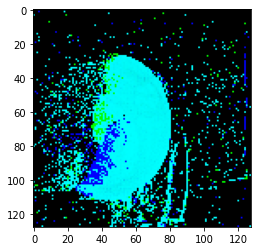
\includegraphics[width=0.25\textwidth]{implementation/images/Dvs128_integrated_frame_2.png}}}%
    \qquad
    \subfloat[\centering]{{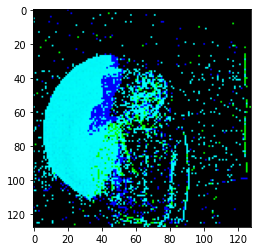
\includegraphics[width=0.25\textwidth]{implementation/images/Dvs128_integrated_frame_3.png}}}%
    \caption{Three contiguous intensity frames ({a}, {b} and {c}), created from the DVS128 Gesture dataset with a person moving their right hand clockwise.}%
    \label{fig:dvs128_integrated_frames}%
\end{figure}

The integratedi frames of a hand gesture in \cref{fig:dvs128_integrated_frames} shows the motion of an arm moving in a clockwise direction. For each instance of a gesture the event stream was split into 20 frames. This made the processing of the data easy for some of the networks described later in the chapter, since the frames could be packed into 3D tensors of equal size. This means that the frames are not synchronous like they would be from an frame-based camera, and the amount of time represented by each frame is varying. As well as this, since the event streams are of varying length in the time dimension, some videos are reconstructed to a more granular scale than others. It is apparent that in this particular sample a relatively large amount of time is being compressed into every frame, resulting in a large amount of motion being visible. With more frames being created for each sample this problem would be alleviated and more easily distinguishable features may be seen. However if too many frames are taken, not only are processing times greatly increased, events may be sparse and not show any visible pattern in any one frame. A benefit of having this blurring event in the intensity frames is that the direction and degree of motion can be seen in the frames, and so the networks can also pick up these patterns in their classification process.

\color{red} TODO: Add more photos of integrated frames with more and less frames \color{black}

\color{red} TODO: Include image and explanations of frame integration \color{black}

\color{red} TODO: Add stuff about possible nlp-like networks. \color{black}

\subsubsection{Time-relative Event Segmentation}
In order to begin analysing neuromorphic data, it was pre-processed it into a form that a NN can take as input. One such method of doing so was to segment the events into groups based on their timestamp. \Cref{fig:nmnist_spikes_to_intensity_map} shows a visualisation of intensity maps created from the NMNIST\cite{NMNIST} dataset. The set of all events was split into eight segments, where each segment included events within a range of $ 1 \times 10^6 $ ms (i.e., $ 0 \rightarrow 1 $, $ 1 \rightarrow 2 $, ..., $ 7 \rightarrow 8 $). This way the data representation shifted to somewhat get back to a set of frames that mimicked the video output usually seen from everyday cameras. \textbf{(a)} shows the segmented events visualised in three dimensions (x\_location, y\_location and timestamp). In \textbf{(b)} these events were projected onto the two dimensional plane (of x\_location and y\_location), then the plots for on events and off events are shown separately. Finally in \textbf{(c)} an intensity map was created from the projected events. Each pixel in the intensity map grid was initialised to 0, and for every on event 1 was added to the cell, and for every off event 1 was subtracted from the cell. It was clear that the resulting output greatly resembled the MNIST\cite{MNIST} sample recorded by the ATIS camera (As shown in \cref{fig:nmnist_spikes_visualisation} in \cref{sec:existing_datasets}).

\begin{figure}[htb]%
    \centering
    \subfloat[\centering]{{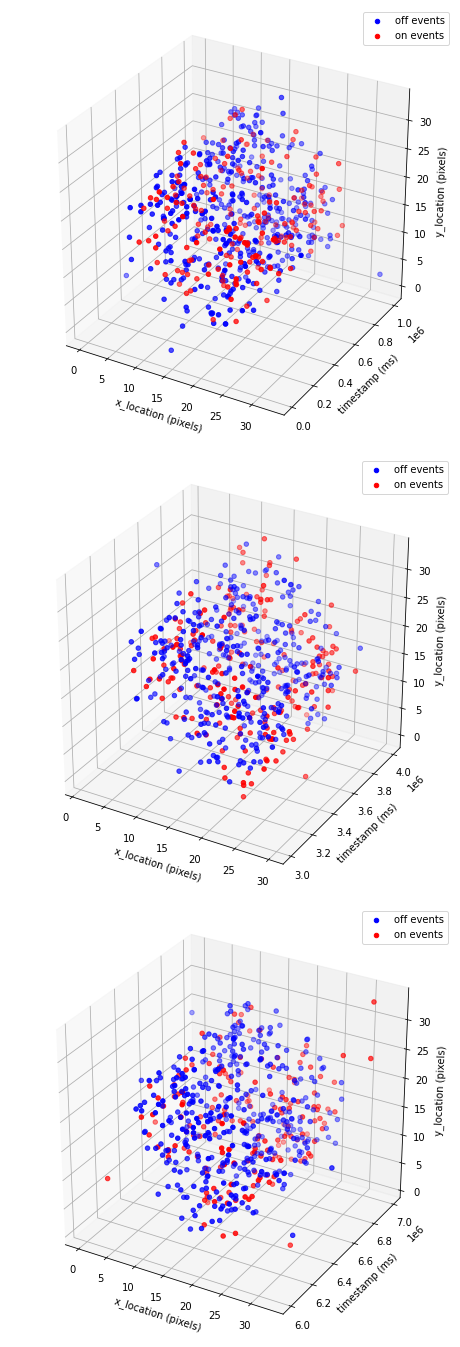
\includegraphics[width=0.25\textwidth, height=0.7\textwidth]{implementation/images/nmnist_spikes_visualisation_segmented.png}}}%
    \qquad
    \subfloat[\centering]{{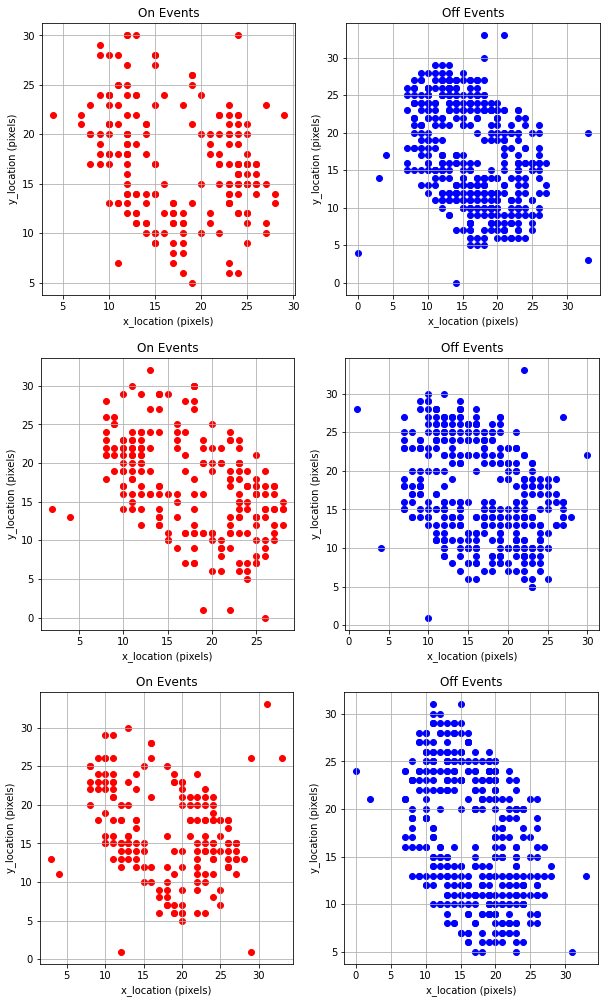
\includegraphics[width=0.4\textwidth, height=0.7\textwidth]{implementation/images/nmnist_events_segmented.png}}}%
    \qquad
    \subfloat[\centering]{{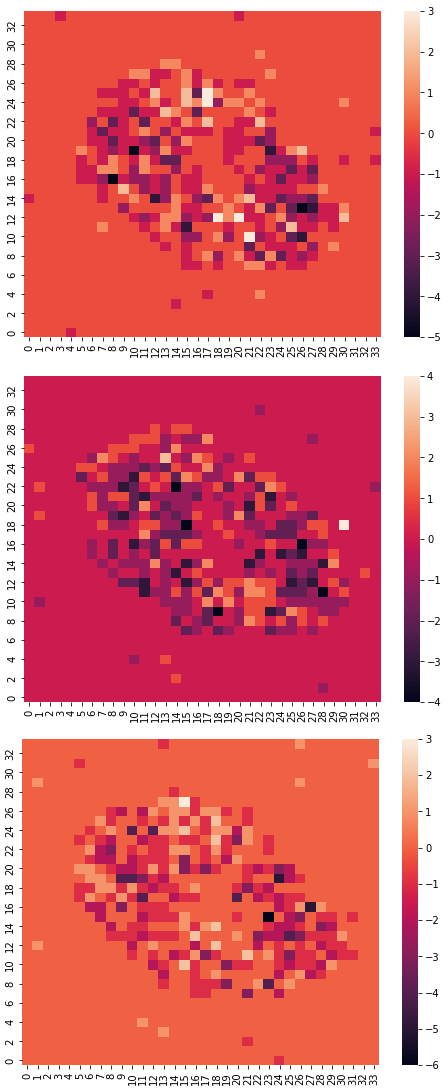
\includegraphics[width=0.25\textwidth, height=0.7\textwidth]{implementation/images/nmnist_events_heatmap_segmented.png}}}%
    \caption{A visualisation of intensity maps created by segmenting events into bins of size $ 1 \times 10^6 $ ms.}%
    \label{fig:nmnist_spikes_to_intensity_map}%
\end{figure}

Once a set of projections was made for each sample from the NMNIST dataset, it could be fed into a neural network in parallel. Ths could be done by simply flattening each intensity map and feeding all the cell values to a fully-connected dense layer in parallel, or the maps could be fed in as images to a convolutional layer. For the convolutional layer method a 3D tensor could be generated by stacking each of the intensity maps against each other and feeding them all directly into the first layer of the NN.

\subsubsection{Neural Network Input Structure}

There were many ways with which a neural network could accept an input to the system. The ones considered for this project where;

\begin{itemize}
    \item Flattening all the intensity maps from segmented event stream into a vector to be input to a single layer of neurons.
    \item Passing a 3D tensor to an convolutional layer as input.
\end{itemize}

\subsection{Classification Models}

\subsubsection{Pure Convolution Network}

The 3D convolutional neural network in \cref{ssec:3D_conv_network} was altered to have the outputs of the hidden layer fed into a dense layer with 10 neurons to classify the correct class (0-9). Activation functions need to be present in the network to prevent all the layers from becoming equivalent to a single one \color{red} TODO: add references here \color{black} (linear regression model). In order to learn more complex patterns activation functions are a necessary aspect of creating an artificial neuron (See \cref{eq:artificial_neuron_output} in \cref{ssec:snn_and_heterogeneity}). The most commonly used activation function in deep networks (and image recognition in particular), and in this network as well, is ReLU. \color{red} TODO: add references here \color{black}. Finally, the output layer has a sigmoid activation function. This function compresses the output smoothly between the ranges of 0 and 1. this means each of the outputs from the neurons can be interpreted as a the probability of the input being any one of the 10 classes. This means we can simply take the highest probability as the predicted class from the network.

Hyper-parameter Tuning:

In order to choose the most appropriate parameters for the system, multiple tests were run varying each of the possible hyper-parameters. The tests conducted were to determine;

\begin{itemize}
    \item The number of hidden layers.
    \item The number of neurons per layer.
    \item The size of convolution kernels.
    \item The introduction of some fully connected layers after convolutional layers.
\end{itemize}

The network in each case was trained for multiple epochs. The performance of a typical network can be seen in \cref{fig:accuracy_and_loss_per_epoch}, where the performance on the training set steadily improves as the network progresses through epochs. Accuracy is one of the metrics defined in \cref{sec:evalutaion_metrics}, and the loss for the given network is called categorical cross-entropy loss. The formula used to calculate the loss is given by: $ L = -\frac{1}{N}\sum^N_{i=1}\sum^C_{c=1}y_c^{(i)}log(\hat{y}_c^{(i)}) $, where there are $ N $ samples and $ C $ classes. $ y_c^{(i)} $ is $ 1 $ when the class is correctly predicted and $ 0 $ otherwise and $ \hat{y}_c^{(i)} $ is the predicted probability of class $ c $ for data-point $ i $.

\begin{figure}[htb]
    \centering
    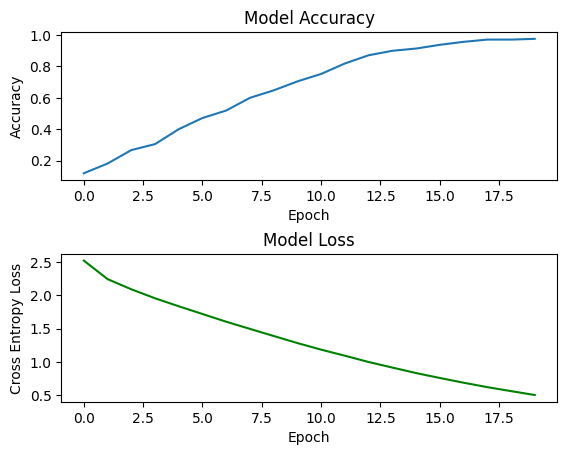
\includegraphics[width=0.4\textwidth]{implementation/images/accuracy_and_loss_per_epoch.png}
    \caption{A figure showing classification accuracy and cross-entropy loss per epoch on training data for a typical network.}
    \label{fig:accuracy_and_loss_per_epoch}
\end{figure}

It was clear, however, that these results may be misleading since they only represent the efficiency of the system when classifying values within the training data-set. However, when looking at the performance on an unseen test data-set, it is obvious that some of the features learnt do not easily translate to general trends in unseen data. This is known as over-fitting, and can be avoided by reducing the capacity of the data-set so that it does not learn information specific to the training set.

Model capacity is directly correlated to the n$ ^o $ of filters, as well as the number of layers, and as the model recognises more patterns in the training data, so it is important to get the optimum value for the system. The size of the kernels has an effect on the scale of the information picked up by the system. With smaller kernels more local patterns are detected, whereas with larger kernels more global effects can be seen \color{red} TODO: add image and reference here \color{black}. As for the dense layers at the end of the network, it can be seen that better results were achieved as a result of it since global patterns can be further identified after the data has been processed by the convolution layers that have picked out the most important features.

\begin{figure}[htb]%
    \centering
    \subfloat[\centering]{{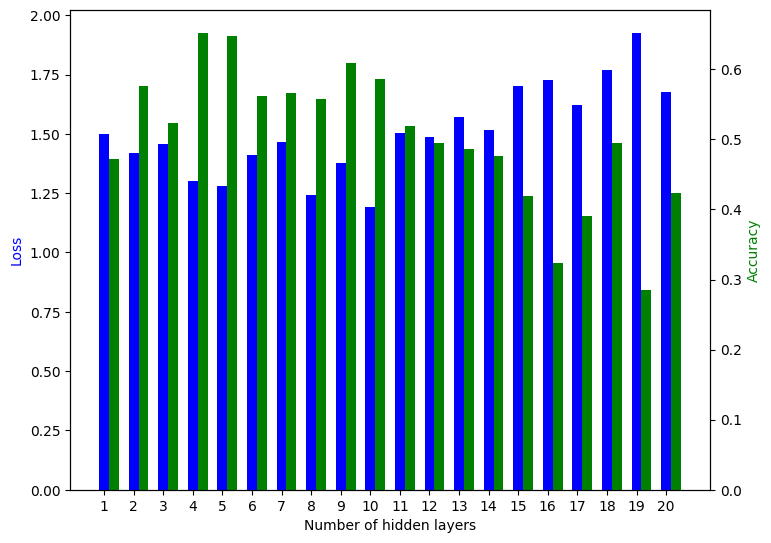
\includegraphics[width=0.4\textwidth]{implementation/images/layer_tests.png}}}%
    \subfloat[\centering]{{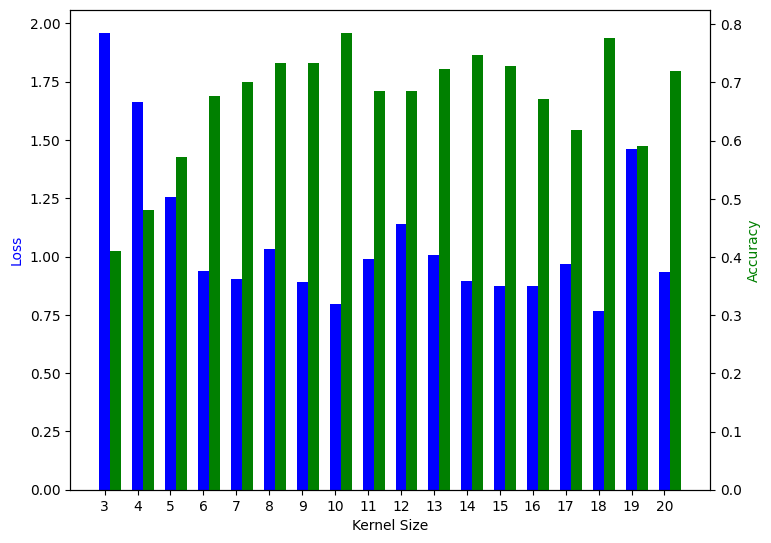
\includegraphics[width=0.4\textwidth]{implementation/images/kernel_tests.png}}}%
    \hfill
    \subfloat[\centering]{{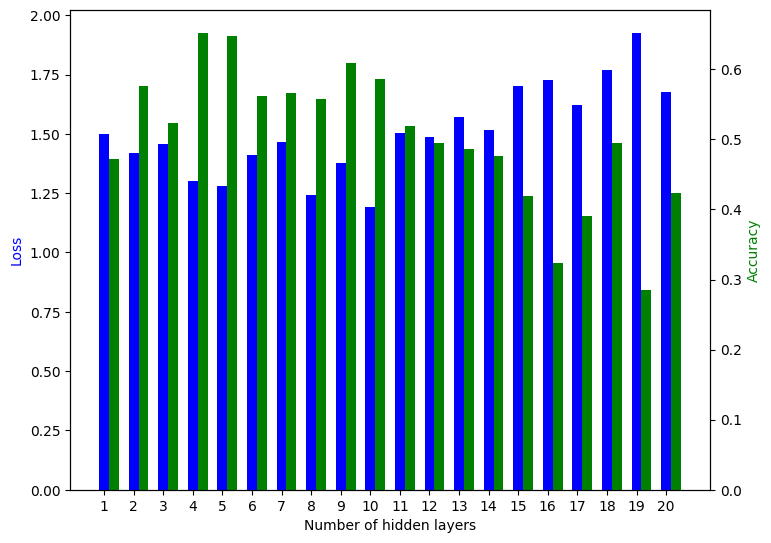
\includegraphics[width=0.4\textwidth]{implementation/images/layer_tests.png}}}%
    \subfloat[\centering]{{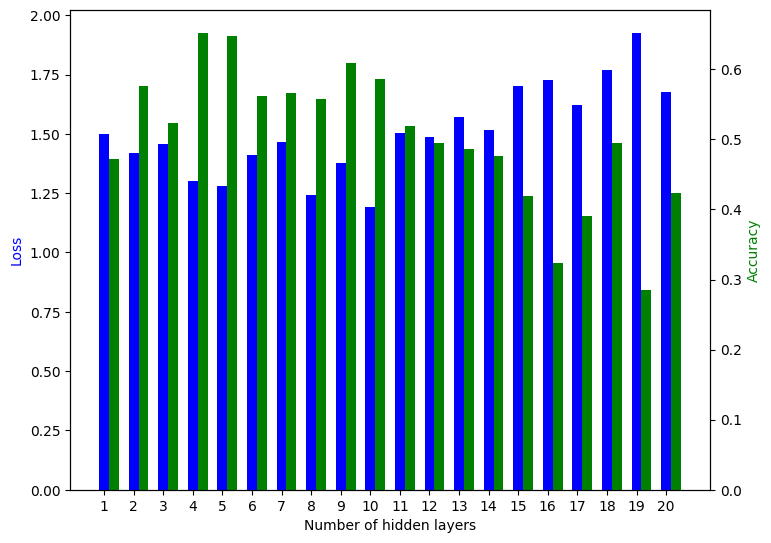
\includegraphics[width=0.4\textwidth]{implementation/images/layer_tests.png}}}%
    \caption{A visualisation of intensity maps created by segmenting events into bins of size $ 1 \times 10^6 $ ms.}%
    \label{fig:tests}%
\end{figure}

Further testing was done with increasing kernel sizes, and with pooling layers added to the network. To find local patters filter kernels smaller than the image (32x32) are used. In earlier layers the no of filters is
large and the filter size is small to capture details. The no
of filters decreases and the filter size increases later in the
network for higher-level patterns. Pooling filters the image
after convolution layers to pick out important features. \color{red} TODO: add final system architecture here \color {black}.

\subsubsection{LTSM}

\subsubsection{Convolutional LTSM}

\color{red} TODO: Show model of custom Conv3D network \color{black}

\section{Spiking Neural Network}

\color{red} TODO: Cite nengo etc. \color{black}

\subsection{Synaptic Smoothing}

\subsection{Firing Rates}

\subsubsection{Post-training Scaling}

\subsubsection{Regularizing During Training}
\chapter{Testing and Results} \label{chap:testing_and_results}

In order to evaluate each of the networks implemented in the previous chapter, various tests were conducted. The main forms of evaluation were previously outlines in \cref{sec:evalutaion_metrics}, allowing for a comprehensive understanding of network performance. As well as this some explanation of the findings are also given.

\section{Data Pre-processing}

The data was converted to the z-score as described in \cref{ssec:data_preprocessing_design}, which made the network learn more stably and ensure any patterns found were more robust and easily applicable to unseen data. This effect was much more apparent on the reconstructed video sequences since the intensities tended to vary much more than the intensities from integrated frames. This is since the values from the integrated frames were naturally `centred' around similar values.

\section{End-to-end Event Classification Models}

The benefits of the event driven camera (as described in \cref{ssec:event_camera_benefits}) were evident in the acquired results. \color{red} TODO: Add images of integrated frames here \color{black}. As opposed to tradition frame-based cameras, high frequency data is not lost when processing events. There are spikes for every event at a much more granular scale in the temporal dimension in the event camera when compared to the frame camera, meaning fast movements were captured more reliably since events are captured at the $\mu s$ scale, no longer restricted by the frame-rates of modern cameras (which often results in motion blur).

\subsection{Frame Integration}

It is, however, evident that modern computer vision techniques have been developed with frame-based cameras in mind, and so modern networks achieve good accuracy, and are able to find patterns well, on frame-based data. For this reason the common technique of integrating frame \color{red} TODO: Add reference to spikingjelly integrating frames from background reading here \color{black} results in regular frames, akin to the ones a regular camera generates, in order to feed into such networks. It does, however, still pose many benefits when compared to the frames from a regular camera. As mentioned previously information between frames is still not lost or degraded since the events are still captured and visible in each frame. As well as this, the frames generated from events inherently focussed on the points of interest in the image, since these were the only ones in motion in the frame. Most common architectures \color{red} TODO: Add references to common gesture recognition architectures here \color{black} for classical videos feature an intermediate layer to remove backgrounds and other noise from images from the image to focus on the points of interest. In this way the intermediate layer could be omitted when operating on the integrated event frames, since the output was already similar to an edge map \color{red} TODO: Add image comparison here \color{black}. It is conceivable, however, that in noisy environments with lots of motion this stage would still be necessary.

It was also interesting to note the inherent ability of neuromorphic cameras to capture points of interest. When using the frame integration method, the result was very similar to an edge map, which is often the primary step of image analysis using convolutional neural networks to images in existing networks already. \Cref{fig:canny_edge_detection_nmnist} shows the effect of carrying out canny edge detection\cite{CannyEdgeDetection} on an integrated frame from the NMNIST dataset. The sample is taken from a recording of the number `0', and it can be seen that the original frame is in essence just a noisy edge map of the number. The steps taken for canny edge detection were as follows;

\begin{enumerate}
    \item Smooth image by convolving with an averaging filter of the form: $ \begin{bmatrix}
        \frac{1}{4^2} & \frac{1}{4^2}  & \frac{1}{4^2}  & \frac{1}{4^2} \\
        \frac{1}{4^2} & \frac{1}{4^2}  & \frac{1}{4^2}  & \frac{1}{4^2} \\
        \frac{1}{4^2} & \frac{1}{4^2}  & \frac{1}{4^2}  & \frac{1}{4^2} \\
        \frac{1}{4^2} & \frac{1}{4^2}  & \frac{1}{4^2}  & \frac{1}{4^2} \\
    \end{bmatrix} $
    \item Sobel edge detection was carried out in order to find the edges of the smoothed image. To do this the image was convolved with the following matrices: $ S_x =
    \begin{bmatrix}
        -1 & 0 & 1 \\
        -2 & 0 & 2 \\
        -1 & 0 & 1 \\
    \end{bmatrix} $ and $ S_y = 
    \begin{bmatrix}
        1 & 2 & 1 \\
        0 & 0 & 0 \\
        -1 & -2 & -1 \\
    \end{bmatrix} $. These matrices got the pixel gradients in the x and y directions, and taking their magnitudes ( $ \sqrt{S_x^2 + S_y^2} $ ) gives the edges map of the frame.
    \item Hysteresis thresholding allowed for weaker edges to be counted as long as they are connected to stronger ones. Then non-maximum suppression was applied to get a single line for every edge (by finding the strongest point of every line in the direction of its gradient).
\end{enumerate}

This refined edge map could have been part of the pre-processing of the data before being passed into the network, but it was found that this was not beneficial to network training. This was because some information is lost in the smoothing process, and any feature mapping was done efficiently during the training of convolutional networks anyway.

\begin{figure}[htb]%
    \centering
    \subfloat[\centering]{{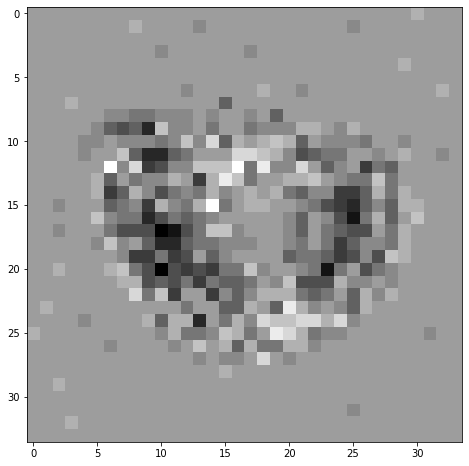
\includegraphics[width=0.18\textwidth]{testingandresults/images/denoise_origional.png}}}%
    \qquad
    \subfloat[\centering]{{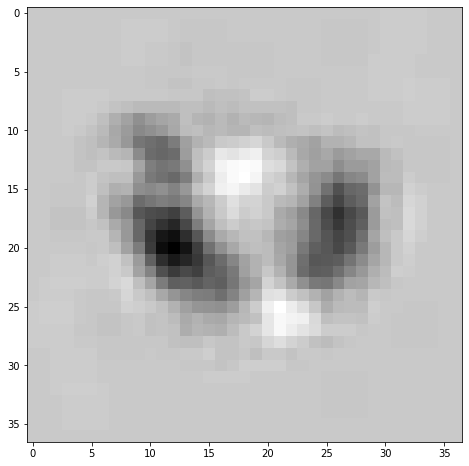
\includegraphics[width=0.18\textwidth]{testingandresults/images/denoise_smoothed.png}}}%
    \qquad
    \subfloat[\centering]{{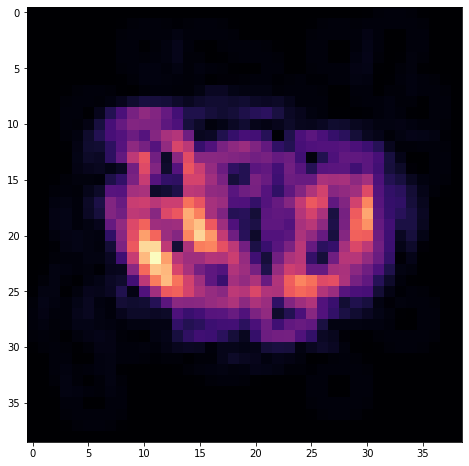
\includegraphics[width=0.18\textwidth]{testingandresults/images/denoise_edge_map.png}}}%
    \qquad
    \subfloat[\centering]{{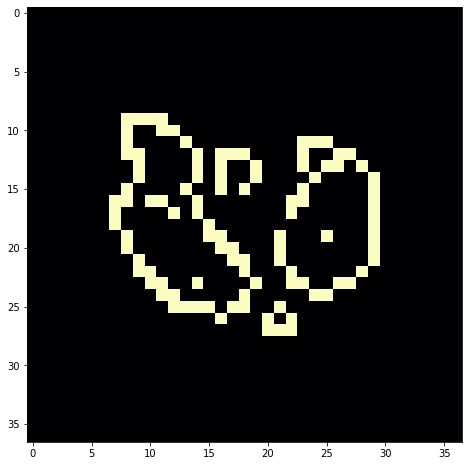
\includegraphics[width=0.18\textwidth]{testingandresults/images/denoise_hysteresis.png}}}%
    \caption{Progression of canny edge detection on integrated frame of a sample from the NMNIST dataset with class `0'. The steps are as follows; \textbf{(a)} original integrated frame, \textbf{(b)} smoothed, \textbf{(c)} edge detection, and \textbf{(d)} Non-maximum suppression and hysteresis thresholding.}%
    \label{fig:canny_edge_detection_nmnist}%
\end{figure}

\color{red} TODO: Write about the two different frame integration methods and show diagrams. \color{black}

\color{red} TODO: Write about the performance difference between synchronous and asynchronous frame integration \color{black}

\section{Two-phase Intensity Reconstruction Models}

\color{red} TODO: Write a nice intro to this section like the last section. \color{black}

\subsection{Intensity Reconstruction}

The E2VID reconstruction network (as described in \cref{ssec:video_reconstruction}) was used to recreate intensity videos from events. It was evident that the reconstructions created were robust and relatively to to life. The reconstructions were not effected by adverse lighting effects or fast motions \color{red} TODO: Add image examples \color{black}. This meant that modern computer vision techniques could still be applied to event data, while still preserving the many benefits the event model presents. It was interesting to note the performance of the reconstruction model on inputs with few moving parts. Since events are only triggered when there is an intensity change on any given pixel on the sensor, only regions with motion in them showed up as events, and the nature of all the space with no motion was not easily inferable. This can clearly be seen in \cref{fig:wave_in_lightings_reconstructions}, where only parts of the scene were accurately reconstructed. This did not, however, pose much of a problem for tasks such as gesture recognition, since the motion is exactly what is being classified, however for other tasks such as object recognition it had to be ensured that there was some sort of motion of either the object or the camera for the reconstruction algorithm to be effective.

\color{red} TODO: Include image and explanations of NMNIST reconstructions \color{black}

\Cref{fig:wave_in_lightings_reconstructions} shows that event-cameras do indeed allow for higher fidelity video capture in a wider range of lighting conditions that frame-based cameras (as explained in \cref{ssec:event_camera_benefits}). In all lighting conditions the video reconstruction was largely the same, since the events triggered were very similar in all cases. The logarithmic characteristics of the event-sensor pixels are the reason for this, since the thresholds for the triggering of events is not static. Since the reconstructions are consistent across lighting conditions, this also means that the reconstruction is more reliable, and the classification algorithm works better in adverse conditions in general \color{red} TODO: get figures and images to prove this \color{black}.

\begin{figure}[htb]%
    \centering
    \subfloat[\centering]{{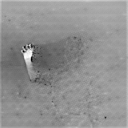
\includegraphics[width=0.18\textwidth]{testingandresults/images/dvs_wave_fluorescent_led.png}}}%
    \qquad
    \subfloat[\centering]{{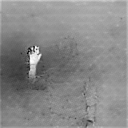
\includegraphics[width=0.18\textwidth]{testingandresults/images/dvs_wave_fluorescent.png}}}%
    \qquad
    \subfloat[\centering]{{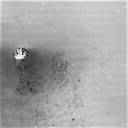
\includegraphics[width=0.18\textwidth]{testingandresults/images/dvs_wave_lab.png}}}%
    \qquad
    \subfloat[\centering]{{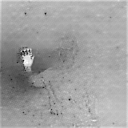
\includegraphics[width=0.18\textwidth]{testingandresults/images/dvs_wave_led.png}}}%
    \qquad
    \subfloat[\centering]{{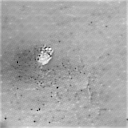
\includegraphics[width=0.18\textwidth]{testingandresults/images/dvs_wave_natural.png}}}%
    \caption{A waving motion being reconstructed from events captures by DVS128 event camera under different lighting conditions.The lighting conditions are as follows; \textbf{(a)} fluorescent led, \textbf{(b)} fluorescent, \textbf{(c)} lab lighting, \textbf{(d)} led lighting and \textbf{(e)} natural lighting.}%
    \label{fig:wave_in_lightings_reconstructions}%
\end{figure}

\subsection{Classification Results}

\subsubsection{NMNIST Dataset}

The confusion matrices for the classification of the NMNIST dataset can be seen in \cref{fig:nmnist_c_matrices}. In terms of precision of classification, all networks perform relatively well. However, the 3D convolutional network and the custom convolutional LSTM network were marginally more effective, achieving a higher accuracy and correctly classifying more challenging event streams. Where this is most apparent is when classifying numbers such as 3, since with the base convolutional LSTM network these were sometime misclassified as an 8 or 9. 

The drawback to the 3D convolutional network is that the number of trainiable parameters (as can be seen in \cref{ssec:conv_3d_network_design}) is much higher than the other networks, and so the training and inference times were considerably higher than the other networks as well (as can be seen in \cref{tab:network_training_times}).

\begin{figure}[htb]%
    \centering
    \subfloat[\centering]{{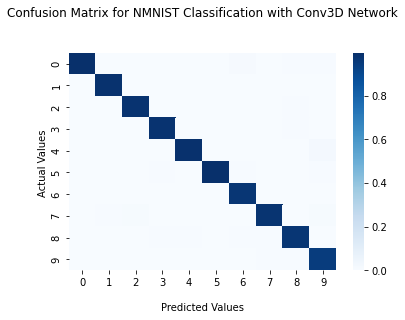
\includegraphics[width=0.4\textwidth]{testingandresults/images/c_matrix_nmnist_conv3d.png}}}%
    \qquad
    \subfloat[\centering]{{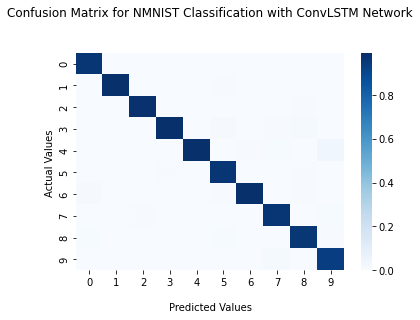
\includegraphics[width=0.4\textwidth]{testingandresults/images/c_matrix_nmnist_convlstm.png}}}%
    \qquad
    \subfloat[\centering]{{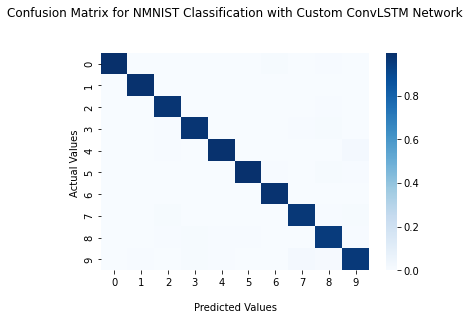
\includegraphics[width=0.4\textwidth]{testingandresults/images/c_matrix_nmnist_custom_convlstm.png}}}%
    \caption{Confusion matrices for NMNIST classification with various networks; \textbf{(a)} conv3D, \textbf{(b)} convLSTM, \textbf{(c)} custom convLSTM.}%
    \label{fig:nmnist_c_matrices}%
\end{figure}

\Cref{tab:conv3d_nmnist_evaluation_metrics}, \cref{tab:conv_lstm_nmnist_evaluation_metrics}, and \cref{tab:custom_conv_lstm_nmnist_evaluation_metrics} show the performance evaluation of each of the networks on the frame-integrated NMNIST dataset in more detail.

\Cref{tab:conv3d_nmnist_recon_evaluation_metrics}, \cref{tab:conv_lstm_nmnist_recon_evaluation_metrics}, and \cref{tab:custom_conv_lstm_nmnist_recon_evaluation_metrics} show the performance evaluation of each of the networks on the intensity reconstructed NMNIST dataset in more detail.

\color{red} TODO: Write more about the meaning of the tables. \color{black}

\color{red} TODO: Make more custom convolution LSTMs \color{black}

\subsubsection{DVS128 Gesture Dataset}

The confusion matrices for the classification of the DVS128 Gesture dataset can be seen in \cref{fig:dvs128_c_matrices}. The variance in performance between the networks is more apparent in this dataset than for the NMNIST dataset. The reason for this is that not only is object detection (of the human body) being undertaken by the system, but also action recognition across frames. It is evident that actions 4 and 5 (right arm clockwise and right arm counter-clockwise), as well as actions 6 and 7 (left arm clockwise and left arm counter-clockwise), were often misclassified as one another. The reason for this was that with length 20 frame integrated videos the fast rotational movement results in frames that look very similar in both directions. \color{red} TODO: Maybe try to get some pictures to prove this. \color{black} Other mistakes were more often made with the 3D convolutional network. For example 10 (air guitar) was quite often predicted for cases of classes 8 and 9 (air roll and air drums). 

\begin{figure}[htb]%
    \centering
    \subfloat[\centering]{{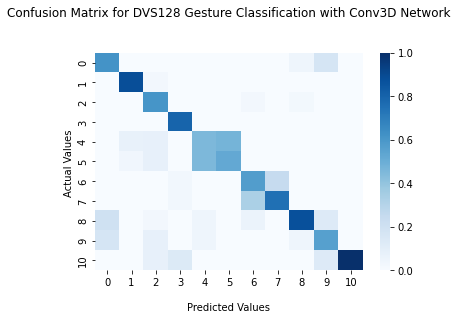
\includegraphics[width=0.4\textwidth]{testingandresults/images/c_matrix_dvs128_conv3d.png}}}%
    \qquad
    \subfloat[\centering]{{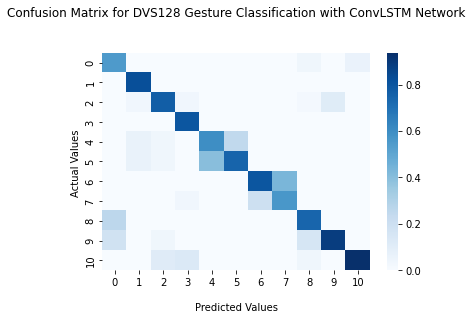
\includegraphics[width=0.4\textwidth]{testingandresults/images/c_matrix_dvs128_convlstm.png}}}%
    \qquad
    \subfloat[\centering]{{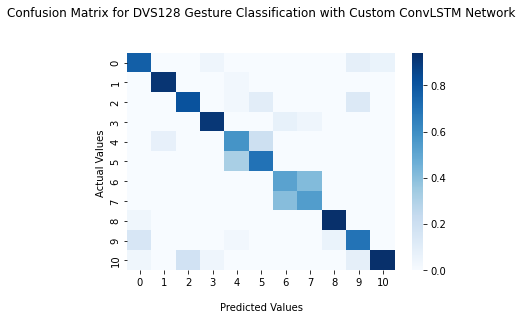
\includegraphics[width=0.4\textwidth]{testingandresults/images/c_matrix_dvs128_custom_convlstm.png}}}%
    \caption{Confusion matrices for DVS128 Gesure classification with various networks; \textbf{(a)} conv3D, \textbf{(b)} convLSTM, \textbf{(c)} custom convLSTM.}%
    \label{fig:dvs128_c_matrices}%
\end{figure}

\Cref{tab:conv3d_dvs128_evaluation_metrics}, \cref{tab:conv_lstm_dvs128_evaluation_metrics}, and \cref{tab:custom_conv_lstm_dvs128_evaluation_metrics} show the performance evaluation of each of the networks on the DVS128 Gesture dataset in more detail.
\color{red} TODO: Write more about the meaning of the tables. \color{black}
\color{red} TODO: Make more custom convolution LSTMs \color{black}

\subsection{Network Comparisons}

\begin{table}[htb]
    \centering
    \begin{tabular}{|| c | c | c ||}
        \hline
        Network     & NMNIST & DVS128 Gesture \\
        \hline \hline
        Conv3D Event Classifier          & 98.22\%   &   69.44\%    \\
        \hline
        Conv2D LTSM Event Classifier         & 97.48\%   &    71.53\%    \\
        \hline
        Custom LTSM Event Classifier         & 97.88\%  &   76.39\%     \\
        \hline
        Conv3D Reconstruction Classifier           & 85.73\%    &       \\
        \hline
        Conv2D LTSM Reconstruction Classifier          & 75.07\%   &      \\
        \hline
        Custom LTSM Reconstruction Classifier         & 80.40\%  &      \\
        \hline
    \end{tabular}
    \caption{A table showing classification accuracies of various models.}
    \label{tab:network_performances}
\end{table}

The full table of classification accuracies can be seen in \cref{tab:network_performances}. Here, the different strengths of the various networks becomes apparent in this comparison. For the simple object classification task on the NMNIST dataset, the higher capacity 3D convolutional network outperformed the others. However, in the more complex task of gesture recognition on the DVS128 Gesture dataset it struggled. The reason for this is that though it is excellent at detecting spacial patterns in each frame, it is less able to detect the temporal patterns prevalent in the gestures.

\begin{table}[htb]
    \centering
    \begin{tabular}{|| c | c | c ||}
        \hline
        Network     & NMNIST & DVS128 Gesture \\
        \hline \hline
        Conv3D Event Classifier          & 1h43m03s   &   0h34m49s    \\
        \hline
        Conv2D LTSM Event Classifier         & 1h03m09s   &    0h08m33s    \\
        \hline
        Custom LTSM Event Classifier         &  1h12m10s  &    \color{red} 1h24m19s \color{black}    \\
        \hline
        Conv3D Reconstruction Classifier        &  0h05m02s    &      \\
        \hline
        Conv2D LTSM Reconstruction Classifier        &  0h14m28s    &      \\
        \hline
        Custom Conv2D LTSM Reconstruction Classifier         &  0h03m26s \color{red} why so short \color{black}  &       \\
        \hline
    \end{tabular}
    \caption{A table showing training times various models.}
    \label{tab:network_training_times}
\end{table}


The training times for each of the networks on the datasets can be seen in \cref{tab:network_training_times}. It is evident that the networks with a higher capacity had higher training times. The 3D convolution network in particular had much longer training times than the other two networks, since it had many more parameters to optimise via back-propagation. It should be noted that for the networks in \color{red} red \color{black} the system encountered an Out Of Memory (OOM) error when attempting create a tensor of larger batch size. For these cases a smaller batch size was used, resulting in slightly higher training times, as well as possible skewed results.
\chapter{Conclusion and Further Work} \label{chap:conclusion_and_further_work}

To conclude, the testing done with the two classification pipelines shows that there are significant benefits to working within the neuromorphic paradigm as opposed to classic frame-based cameras. With the same networks, performance appears to be superior when analysing event streams rather than video frames for simple object recognition and classification tasks. Secondly, the two-phase intensity reconstruction pipelines show promise, being able to harness the wealth of existing networks that exist for video classification. 

The performance with the same classification networks directly on the events rather than the video reconstructions tended to have better performance for simple object recognition and classification tasks. This is perhaps due to the loss of high-frequency data and when creating the intensity maps. However, this was not the case for more complex tasks such as gesture recognition. In this case the reconstructions were found to be of superior quality (perhaps due to the size and nature of the dataset used), allowing for better analysis of the recorded gestures. 

The reconstructions show that the benefits of event-based cameras can be retained even when working with intensity videos, as the reconstruction networks produce high fidelity outputs even when recording videos with lots of motion or high dynamic range of light intensities. This means that the reconstructed videos are often more appropriate for classification that if a video was taken with a frame-based camera. 

Finally, testing the conversion of a 3D convolutional network showed that equivalent performance could be attained, while harnessing the benefits of spiking neural networks. Close to 100\% of the performance of the non-spiking equivalent was achieved while having a spiking rate of below 1Hz. This is beneficial since the information being passed between the layers of the neural network are now sparse, meaning less communication needs to take place overall to analyse the data. This is therefore a much less power intensive, and more computationally efficient encoding affording itself to the use on low-powered chips and for real-time processing. This is especially true of the fully neuromorphic system detailed in this report, since the input is from a event-based camera, which in itself is much more power-efficient than frame-based cameras. The Legendre Memory Unit also shows promise as a good way of implemented a recurrent unit in a spiking neural network, however more work needs to be done to tune the performance.

\section{Further Work}

Having reached the end of the project, it is important to note the limitations (such as computing power and available time) that need to be acknowledged. As such, there are some key areas in which there is scope for further research and development. These include;

\begin{enumerate}
    \item With a more capable setup and time to test the networks, there is the opportunity to create more intensive networks. As well as this larger batch sizes can be used for more stable training with higher RAM available.
    \item Compare the performance of the reconstructed pipeline like-for-like against a video stream from a frame-based camera. This has been omitted from this project due to time constraints and lack of available datasets.
    \item Change E2VID parameters so that resulting reconstructed video is of a higher framerate.
    \item Test the performance of the described networks and pipelines on more readily available datasets to make sure that the findings apply to other environments. Intensity reconstructions may be beneficial for more complex tasks.
    \item Look more at the use of natural language processing techniques such as Bag of Words and Support Vector Machines when working with event streams.
    \item Create more spiking neural networks, perhaps from scratch rather than converting regular ANNs. Further testing needs to be done in this area.
    \item Tune the LMU to work well on the given datasets.
    \item Test performance of spiking neural networks on intensity reconstructed video streams.
    \item Test the performance of the end-to-end event classification networks when frame-integration is done asynchronously as well as synchronously (as described in \cref{ssec:frame_integration}). 
    \item The effect of having smaller time-slices per integrated frame need to be tested, where the data has an equivalent size to the E2VID output.
    \item Create spiking neural networks based on more complex ANN networks. This involves creating approximations to other, more complex layers such as LSTM and GRU layers.
    \item Implement spiking neural networks on neuromorphic hardware. This also opens up the possibility of real-time inference.
    \item Create a spiking version of the intensity reconstruction algorithms to check if they perform well.
\end{enumerate}

\section{Similar External Work}

A method, similar to the custom frame integration proposed in \cref{sssec:custom_frame_integration_implementation}, that aimed to preserve temporal resolution was proposed by Lo\"ic Cordone \textit{et al.}, who proposed `voxel cubes'\cite{MiniVovelCubes}. For this method there were still binary events in every channel, but there were more than two channels so that the events in each time-slice could be subdivided into each channel. When compared to this method, the temporal information can be stored in the same way with the novel method proposed in this project, while keeping data size small since it is just a one-channel image. 

More work by Lo\"ic Cordone \textit{et al.}\cite{OtherSnnWork}, shows testing with sparse SNN architectures (using surrogate training as done in this report) achieving similar performance on the DVS dataset to the networks outlined in this report. In their paper a 2D spiking convolutional neural network is compared to a 3D convolutional network, and the training and inference times are outlines to show the efficiency of spiking encoding.

\appendix
\chapter{Classification Model Architectures}

\begin{lstlisting}[language=Bash,caption={Overview of layers in 3D convolutional network},label={lst:3d_conv_layers},numbers=none,float=htb]
_________________________________________________________________
Layer (type)                Output Shape              Param #   
=================================================================
conv3d_10 (Conv3D)          (None, 8, 34, 34, 32)     4032      
                                                                
batch_normalization_12 (Bat  (None, 8, 34, 34, 32)    128       
chNormalization)                                                
                                                                
conv3d_11 (Conv3D)          (None, 8, 34, 34, 32)     128032    
                                                                
batch_normalization_13 (Bat  (None, 8, 34, 34, 32)    128       
chNormalization)                                                
                                                                
max_pooling3d_6 (MaxPooling  (None, 4, 17, 17, 32)    0         
3D)                                                             
                                                                
dropout_8 (Dropout)         (None, 4, 17, 17, 32)     0         
                                                                
conv3d_12 (Conv3D)          (None, 4, 17, 17, 64)     256064    
                                                                
batch_normalization_14 (Bat  (None, 4, 17, 17, 64)    256       
chNormalization)                                                
                                                                
max_pooling3d_7 (MaxPooling  (None, 2, 9, 9, 64)      0         
3D)                                                             
                                                                
dropout_9 (Dropout)         (None, 2, 9, 9, 64)       0         
                                                                
conv3d_13 (Conv3D)          (None, 2, 9, 9, 128)      1024128   
                                                                
batch_normalization_15 (Bat  (None, 2, 9, 9, 128)     512       
chNormalization)                                                
                                                                
conv3d_14 (Conv3D)          (None, 2, 9, 9, 128)      2048128   
                                                                
batch_normalization_16 (Bat  (None, 2, 9, 9, 128)     512       
chNormalization)                                                
                                                                
max_pooling3d_8 (MaxPooling  (None, 1, 5, 5, 128)     0         
3D)                                                             
                                                                
dropout_10 (Dropout)        (None, 1, 5, 5, 128)      0         
                                                                
flatten_2 (Flatten)         (None, 3200)              0         
                                                                
dense_4 (Dense)             (None, 128)               409728    
                                                                
batch_normalization_17 (Bat  (None, 128)              512       
chNormalization)                                                
                                                                
dropout_11 (Dropout)        (None, 128)               0         
                                                                
dense_5 (Dense)             (None, 10)                1290      
                                                                
activation_2 (Activation)   (None, 10)                0         
                                                                
=================================================================
Total params: 3,873,450
Trainable params: 3,872,426
Non-trainable params: 1,024
_________________________________________________________________
\end{lstlisting}

\begin{lstlisting}[language=Bash,caption={Overview of layers in Convolutional LTSM network.},label={lst:conv_lstm_layers},numbers=none,float=htb]
_________________________________________________________________
Layer (type)                Output Shape              Param #   
=================================================================
conv_lstm2d_6 (ConvLSTM2D)  (None, 8, 34, 34, 64)     150016    
                                                                
max_pooling3d_4 (MaxPooling  (None, 8, 17, 17, 64)    0         
3D)                                                             
                                                                
batch_normalization_6 (Batc  (None, 8, 17, 17, 64)    256       
hNormalization)                                                 
                                                                
conv_lstm2d_7 (ConvLSTM2D)  (None, 8, 17, 17, 32)     110720    
                                                                
max_pooling3d_5 (MaxPooling  (None, 8, 9, 9, 32)      0         
3D)                                                             
                                                                
batch_normalization_7 (Batc  (None, 8, 9, 9, 32)      128       
hNormalization)                                                 
                                                                
conv_lstm2d_8 (ConvLSTM2D)  (None, 9, 9, 16)          27712     
                                                                
max_pooling2d_2 (MaxPooling  (None, 5, 5, 16)         0         
2D)                                                             
                                                                
batch_normalization_8 (Batc  (None, 5, 5, 16)         64        
hNormalization)                                                 
                                                                
flatten_2 (Flatten)         (None, 400)               0         
                                                                
dense_4 (Dense)             (None, 256)               102656    
                                                                
dense_5 (Dense)             (None, 10)                2570      
                                                                
=================================================================
Total params: 394,122
Trainable params: 393,898
Non-trainable params: 224
_________________________________________________________________
\end{lstlisting}

\begin{lstlisting}[language=Bash,caption={Overview of layers in Custom Convolutional LTSM network.},label={lst:custom_conv_lstm_layers},numbers=none,float=htb]
_________________________________________________________________
Layer (type)                Output Shape              Param #   
=================================================================
time_distributed_3 (TimeDis  (None, 8, 2048)          4887936   
tributed)                                                       
                                                                
gru_3 (GRU)                 (None, 64)                405888    
                                                                
dense_25 (Dense)            (None, 1024)              66560     
                                                                
dropout_9 (Dropout)         (None, 1024)              0         
                                                                
dense_26 (Dense)            (None, 512)               524800    
                                                                
dropout_10 (Dropout)        (None, 512)               0         
                                                                
dense_27 (Dense)            (None, 128)               65664     
                                                                
dropout_11 (Dropout)        (None, 128)               0         
                                                                
dense_28 (Dense)            (None, 64)                8256      
                                                                
dense_29 (Dense)            (None, 10)                650       
                                                                
=================================================================
Total params: 5,959,754
Trainable params: 5,959,754
Non-trainable params: 0
_________________________________________________________________
\end{lstlisting}

\begin{lstlisting}[language=Bash,caption={Overview of layers in Custom 2D Convolutional network built into the Custom LSTM Network in \cref{lst:custom_conv_lstm_layers}.},label={lst:custom_conv_2d_layers},numbers=none,float=htb]
_________________________________________________________________
Layer (type)                Output Shape              Param #   
=================================================================
conv2d_3 (Conv2D)           (None, 34, 34, 128)       640       
                                                                
activation_3 (Activation)   (None, 34, 34, 128)       0         
                                                                
max_pooling2d_4 (MaxPooling  (None, 17, 17, 128)      0         
2D)                                                             
                                                                
conv2d_4 (Conv2D)           (None, 17, 17, 256)       131328    
                                                                
activation_4 (Activation)   (None, 17, 17, 256)       0         
                                                                
max_pooling2d_5 (MaxPooling  (None, 8, 8, 256)        0         
2D)                                                             
                                                                
conv2d_5 (Conv2D)           (None, 8, 8, 512)         524800    
                                                                
activation_5 (Activation)   (None, 8, 8, 512)         0         
                                                                
max_pooling2d_6 (MaxPooling  (None, 4, 4, 512)        0         
2D)                                                             
                                                                
flatten_2 (Flatten)         (None, 8192)              0         
                                                                
dense_7 (Dense)             (None, 256)               2097408   
                                                                
activation_6 (Activation)   (None, 256)               0         
                                                                
dense_8 (Dense)             (None, 10)                2570      
                                                                
activation_7 (Activation)   (None, 10)                0         
                                                                
=================================================================
Total params: 2,756,746
Trainable params: 2,756,746
Non-trainable params: 0
_________________________________________________________________
\end{lstlisting}
\chapter{Evaluation Metrics of Each Trained Model}

\begin{table}[htb]
    \centering
    \begin{tabular}{|| c | c | c | c | c ||}
        \hline
             & Precision & Recall & F1-score & Samples \\
        \hline \hline
        0            & 1.00 & 0.99 & 0.99 & 500  \\
        \hline
        1            & 0.99 & 1.00 & 0.99 & 500  \\
        \hline
        2            & 0.99 & 0.99 & 0.99 & 500  \\
        \hline
        3            & 0.98 & 1.00 & 0.99 & 500  \\
        \hline
        4            & 0.99 & 0.99 & 0.99 & 500  \\
        \hline
        5            & 0.99 & 0.97 & 0.98 & 500  \\
        \hline
        6            & 0.99 & 0.99 & 0.99 & 500  \\
        \hline
        7            & 0.99 & 0.97 & 0.98 & 500  \\
        \hline
        8            & 0.97 & 0.99 & 0.98 & 500  \\
        \hline
        9            & 0.98 & 0.98 & 0.98 & 500  \\
        \hline
        macro avg    & 0.99 & 0.99 & 0.99 & 5000 \\
        \hline
        weighted avg & 0.99 & 0.99 & 0.99 & 5000 \\
        \hline
    \end{tabular}
    \caption{A table showing classification evaluation metrics of 3D convolutional network on the frame-integrated NMNIST dataset.}
    \label{tab:conv3d_nmnist_evaluation_metrics}
\end{table}

\begin{table}[htb]
    \centering
    \begin{tabular}{|| c | c | c | c | c ||}
        \hline
             & Precision & Recall & F1-score & Samples \\
        \hline \hline
        0            & 0.97 & 1.00 & 0.98 & 500  \\
        \hline
        1            & 0.99 & 0.99 & 0.99 & 500  \\
        \hline
        2            & 0.99 & 0.99 & 0.99 & 500  \\
        \hline
        3            & 0.99 & 0.96 & 0.97 & 500  \\
        \hline
        4            & 0.99 & 0.95 & 0.97 & 500  \\
        \hline
        5            & 0.97 & 0.98 & 0.98 & 500  \\
        \hline
        6            & 0.99 & 0.97 & 0.98 & 500  \\
        \hline
        7            & 0.97 & 0.98 & 0.97 & 500  \\
        \hline
        8            & 0.96 & 0.97 & 0.97 & 500  \\
        \hline
        9            & 0.94 & 0.98 & 0.96 & 500  \\
        \hline
        macro avg    & 0.98 & 0.98 & 0.98 & 5000 \\
        \hline
        weighted avg & 0.98 & 0.98 & 0.98 & 5000 \\
        \hline
    \end{tabular}
    \caption{A table showing classification evaluation metrics of convolutional LSTM network on the frame-integrated NMNIST dataset.}
    \label{tab:conv_lstm_nmnist_evaluation_metrics}
\end{table}

\begin{table}[htb]
    \centering
    \begin{tabular}{|| c | c | c | c | c ||}
        \hline
             & Precision & Recall & F1-score & Samples \\
        \hline \hline
        0            & 0.98 & 0.99 & 0.99 & 500  \\
        \hline
        1            & 0.98 & 0.99 & 0.99 & 500  \\
        \hline
        2            & 0.99 & 0.97 & 0.98 & 500  \\
        \hline
        3            & 0.99 & 0.96 & 0.97 & 500  \\
        \hline
        4            & 0.99 & 0.98 & 0.98 & 500  \\
        \hline
        5            & 0.98 & 0.97 & 0.97 & 500  \\
        \hline
        6            & 0.98 & 0.99 & 0.98 & 500  \\
        \hline
        7            & 0.96 & 0.99 & 0.98 & 500  \\
        \hline
        8            & 0.94 & 0.97 & 0.95 & 500  \\
        \hline
        9            & 0.98 & 0.96 & 0.97 & 500  \\
        \hline
        macro avg    & 0.98 & 0.98 & 0.98 & 5000 \\
        \hline
        weighted avg & 0.98 & 0.98 & 0.98 & 5000 \\
        \hline
    \end{tabular}
    \caption{A table showing classification evaluation metrics of custom convolutional LSTM network on the frame-integrated NMNIST dataset.}
    \label{tab:custom_conv_lstm_nmnist_evaluation_metrics}
\end{table}

\begin{table}[htb]
    \centering
    \begin{tabular}{|| c | c | c | c | c ||}
        \hline
             & Precision & Recall & F1-score & Samples \\
        \hline \hline
        0            & 1.00  & 0.97  & 0.98 & 500 \\
        \hline
        1            & 0.99  & 1.00  & 0.99 & 500 \\
        \hline
        2            & 0.99  & 0.99  & 0.99 & 500 \\
        \hline
        3            & 0.99  & 0.99  & 0.99 & 500 \\
        \hline
        4            & 0.99  & 0.97  & 0.98 & 500 \\
        \hline
        5            & 1.00  & 0.98  & 0.99 & 500 \\
        \hline
        6            & 0.97  & 1.00  & 0.98 & 500 \\
        \hline
        7            & 0.98  & 0.97  & 0.98 & 500 \\
        \hline
        8            & 0.97  & 0.97  & 0.97 & 500 \\
        \hline
        9            & 0.95  & 0.98  & 0.96 & 500 \\
        \hline
        macro avg    & 0.98  & 0.98  & 0.98 & 5000 \\
        \hline
        weighted avg & 0.98  & 0.98  & 0.98 & 5000 \\
        \hline
    \end{tabular}
    \caption{A table showing classification evaluation metrics of 3D convolutional network on the custom frame-integrated NMNIST dataset.}
    \label{tab:conv3d_nmnist_custom_frame_evaluation_metrics}
\end{table}

\begin{table}[htb]
    \centering
    \begin{tabular}{|| c | c | c | c | c ||}
        \hline
             & Precision & Recall & F1-score & Samples \\
        \hline \hline
        0            & 0.99 & 0.99 & 0.99 & 500  \\
        \hline
        1            & 0.98 & 1.00 & 0.99 & 500  \\
        \hline
        2            & 0.97 & 0.99 & 0.98 & 500  \\
        \hline
        3            & 0.94 & 0.99 & 0.96 & 500  \\
        \hline
        4            & 1.00 & 0.98 & 0.99 & 500  \\
        \hline
        5            & 0.96 & 0.99 & 0.98 & 500  \\
        \hline
        6            & 0.99 & 0.99 & 0.99 & 500  \\
        \hline
        7            & 0.96 & 0.98 & 0.97 & 500  \\
        \hline
        8            & 0.98 & 0.91 & 0.95 & 500  \\
        \hline
        9            & 0.97 & 0.94 & 0.96 & 500  \\
        \hline
        macro avg    & 0.98 & 0.97 & 0.97 & 5000 \\
        \hline
        weighted avg & 0.98 & 0.97 & 0.97 & 5000 \\
        \hline
    \end{tabular}
    \caption{A table showing classification evaluation metrics of convolutional LSTM network on the custom frame-integrated NMNIST dataset.}
    \label{tab:conv_lstm_nmnist_custom_frame_evaluation_metrics}
\end{table}

\begin{table}[htb]
    \centering
    \begin{tabular}{|| c | c | c | c | c ||}
        \hline
             & Precision & Recall & F1-score & Samples \\
        \hline \hline
        0            & 0.98 & 0.98 & 0.98 & 500  \\
        \hline
        1            & 0.98 & 1.00 & 0.99 & 500  \\
        \hline
        2            & 0.98 & 0.99 & 0.98 & 500  \\
        \hline
        3            & 0.98 & 0.97 & 0.97 & 500  \\
        \hline
        4            & 0.99 & 0.98 & 0.98 & 500  \\
        \hline
        5            & 0.98 & 0.98 & 0.98 & 500  \\
        \hline
        6            & 0.97 & 0.99 & 0.98 & 500  \\
        \hline
        7            & 0.96 & 0.98 & 0.97 & 500  \\
        \hline
        8            & 0.97 & 0.94 & 0.96 & 500  \\
        \hline
        9            & 0.98 & 0.94 & 0.96 & 500  \\
        \hline
        macro avg    & 0.98 & 0.98 & 0.98 & 5000 \\
        \hline
        weighted avg & 0.98 & 0.98 & 0.98 & 5000 \\
        \hline
    \end{tabular}
    \caption{A table showing classification evaluation metrics of custom convolutional LSTM network on the custom frame-integrated NMNIST dataset.}
    \label{tab:custom_conv_lstm_nmnist_custom_frame_evaluation_metrics}
\end{table}

\begin{table}[htb]
    \centering
    \begin{tabular}{|| c | c | c | c | c ||}
        \hline
             & Precision & Recall & F1-score & Samples \\
        \hline \hline
        0            & 0.94 & 0.96 & 0.95 & 75  \\
        \hline
        1            & 0.95 & 0.96 & 0.95 & 75  \\
        \hline
        2            & 0.85 & 0.93 & 0.89 & 75  \\
        \hline
        3            & 0.84 & 0.71 & 0.77 & 75  \\
        \hline
        4            & 0.93 & 0.84 & 0.88 & 75  \\
        \hline
        5            & 0.71 & 0.87 & 0.78 & 75  \\
        \hline
        6            & 0.87 & 0.91 & 0.89 & 75  \\
        \hline
        7            & 0.91 & 0.85 & 0.88 & 75  \\
        \hline
        8            & 0.86 & 0.73 & 0.79 & 75  \\
        \hline
        9            & 0.85 & 0.91 & 0.88 & 75  \\
        \hline
        macro avg    & 0.87 & 0.87 & 0.87 & 750 \\
        \hline
        weighted avg & 0.87 & 0.87 & 0.87 & 750 \\
        \hline
    \end{tabular}
    \caption{A table showing classification evaluation metrics of 3D convolutional network on the reconstructed NMNIST dataset.}
    \label{tab:conv3d_nmnist_recon_evaluation_metrics}
\end{table}

\begin{table}[htb]
    \centering
    \begin{tabular}{|| c | c | c | c | c ||}
        \hline
             & Precision & Recall & F1-score & Samples \\
        \hline \hline
        0            & 0.83 & 0.92 & 0.87 & 75  \\
        \hline
        1            & 0.96 & 0.96 & 0.96 & 75  \\
        \hline
        2            & 0.82 & 0.91 & 0.86 & 75  \\
        \hline
        3            & 0.77 & 0.57 & 0.66 & 75  \\
        \hline
        4            & 0.74 & 0.72 & 0.73 & 75  \\
        \hline
        5            & 0.67 & 0.71 & 0.69 & 75  \\
        \hline
        6            & 0.88 & 0.85 & 0.86 & 75  \\
        \hline
        7            & 0.85 & 0.84 & 0.85 & 75  \\
        \hline
        8            & 0.74 & 0.64 & 0.69 & 75  \\
        \hline
        9            & 0.71 & 0.84 & 0.77 & 75  \\
        \hline
        macro avg    & 0.80 & 0.80 & 0.79 & 750 \\
        \hline
        weighted avg & 0.80 & 0.80 & 0.79 & 750 \\
        \hline
    \end{tabular}
    \caption{A table showing classification evaluation metrics of convolutional LSTM network on the reconstructed NMNIST dataset.}
    \label{tab:conv_lstm_nmnist_recon_evaluation_metrics}
\end{table}

\begin{table}[htb]
    \centering
    \begin{tabular}{|| c | c | c | c | c ||}
        \hline
             & Precision & Recall & F1-score & Samples \\
        \hline \hline
        0            & 0.88 & 0.95 & 0.91 & 75  \\
        \hline
        1            & 0.99 & 0.92 & 0.95 & 75  \\
        \hline
        2            & 0.93 & 0.85 & 0.89 & 75  \\
        \hline
        3            & 0.79 & 0.76 & 0.78 & 75  \\
        \hline
        4            & 0.96 & 0.73 & 0.83 & 75  \\
        \hline
        5            & 0.71 & 0.81 & 0.76 & 75  \\
        \hline
        6            & 0.81 & 0.92 & 0.86 & 75  \\
        \hline
        7            & 0.82 & 0.84 & 0.83 & 75  \\
        \hline
        8            & 0.68 & 0.68 & 0.68 & 75  \\
        \hline
        9            & 0.82 & 0.85 & 0.84 & 75  \\
        \hline
        macro avg    & 0.84 & 0.83 & 0.83 & 750 \\
        \hline
        weighted avg & 0.84 & 0.83 & 0.83 & 750 \\
        \hline
    \end{tabular}
    \caption{A table showing classification evaluation metrics of custom convolutional LSTM network on the reconstructed NMNIST dataset.}
    \label{tab:custom_conv_lstm_nmnist_recon_evaluation_metrics}
\end{table}

\begin{table}[htb]
    \centering
    \begin{tabular}{|| c | c | c | c | c ||}
        \hline
            & Precision & Recall & F1-score & Samples \\
        \hline
        \hline
        0            & 0.55 & 0.88 & 0.68 & 24  \\
        \hline
        1            & 0.83 & 1.00 & 0.91 & 24  \\
        \hline
        2            & 0.77 & 0.83 & 0.80 & 24  \\
        \hline
        3            & 0.80 & 1.00 & 0.89 & 24  \\
        \hline
        4            & 0.60 & 0.75 & 0.67 & 24  \\
        \hline
        5            & 0.75 & 0.38 & 0.50 & 24  \\
        \hline
        6            & 0.80 & 0.33 & 0.47 & 24  \\
        \hline
        7            & 0.57 & 0.88 & 0.69 & 24  \\
        \hline
        8            & 0.75 & 0.79 & 0.77 & 48  \\
        \hline
        9            & 0.89 & 0.33 & 0.48 & 24  \\
        \hline
        10           & 0.94 & 0.62 & 0.75 & 24  \\
        \hline
        macro avg    & 0.75 & 0.71 & 0.69 & 288 \\
        \hline
        weighted avg & 0.75 & 0.72 & 0.70 & 288 \\
        \hline
    \end{tabular}
    \caption{A table showing classification evaluation metrics of 3D convolutional network on the frame-integrated DVS128 Gesture dataset.}
    \label{tab:conv3d_dvs128_evaluation_metrics}
\end{table}

\begin{table}[htb]
    \centering
    \begin{tabular}{|| c | c | c | c | c ||}
        \hline
             & Precision & Recall & F1-score & Samples \\
        \hline
        \hline
        0            & 0.55 & 0.88 & 0.68 & 24  \\
        \hline
        1            & 0.83 & 1.00 & 0.91 & 24  \\
        \hline
        2            & 0.77 & 0.83 & 0.80 & 24  \\
        \hline
        3            & 0.80 & 1.00 & 0.89 & 24  \\
        \hline
        4            & 0.60 & 0.75 & 0.67 & 24  \\
        \hline
        5            & 0.75 & 0.38 & 0.50 & 24  \\
        \hline
        6            & 0.80 & 0.33 & 0.47 & 24  \\
        \hline
        7            & 0.57 & 0.88 & 0.69 & 24  \\
        \hline
        8            & 0.75 & 0.79 & 0.77 & 48  \\
        \hline
        9            & 0.89 & 0.33 & 0.48 & 24  \\
        \hline
        10           & 0.94 & 0.62 & 0.75 & 24  \\
        \hline
        macro avg    & 0.75 & 0.71 & 0.69 & 288 \\
        \hline
        weighted avg & 0.75 & 0.72 & 0.70 & 288 \\
        \hline
    \end{tabular}
    \caption{A table showing classification evaluation metrics of convolutional LSTM network on the frame-integrated DVS128 Gesture dataset.}
    \label{tab:conv_lstm_dvs128_evaluation_metrics}
\end{table}

\begin{table}[htb]
    \centering
    \begin{tabular}{|| c | c | c | c | c ||}
        \hline
             & Precision & Recall & F1-score & Samples \\
        \hline
        \hline
        0            & 0.77 & 0.83 & 0.80 & 24  \\
        \hline
        1            & 0.92 & 0.96 & 0.94 & 24  \\
        \hline
        2            & 0.82 & 0.75 & 0.78 & 24  \\
        \hline
        3            & 0.91 & 0.88 & 0.89 & 24  \\
        \hline
        4            & 0.58 & 0.75 & 0.65 & 24  \\
        \hline
        5            & 0.70 & 0.58 & 0.64 & 24  \\
        \hline
        6            & 0.52 & 0.58 & 0.55 & 24  \\
        \hline
        7            & 0.54 & 0.54 & 0.54 & 24  \\
        \hline
        8            & 0.94 & 0.98 & 0.96 & 48  \\
        \hline
        9            & 0.70 & 0.67 & 0.68 & 24  \\
        \hline
        10           & 0.94 & 0.67 & 0.78 & 24  \\
        \hline
        macro avg    & 0.76 & 0.74 & 0.75 & 288 \\
        \hline
        weighted avg & 0.77 & 0.76 & 0.76 & 288 \\
        \hline
    \end{tabular}
    \caption{A table showing classification evaluation metrics of a convolutional LSTM on the frame-integratedDVS128 Gesture dataset.}
    \label{tab:custom_conv_lstm_dvs128_evaluation_metrics}
\end{table}

\begin{table}[htb]
    \centering
    \begin{tabular}{|| c | c | c | c | c ||}
        \hline
            & Precision & Recall & F1-score & Samples \\
        \hline \hline
        0            & 0.53 & 0.88 & 0.66 & 24  \\
        \hline
        1            & 0.85 & 0.96 & 0.90 & 24  \\
        \hline
        2            & 0.88 & 0.88 & 0.88 & 24  \\
        \hline
        3            & 0.43 & 0.92 & 0.59 & 24  \\
        \hline
        4            & 0.42 & 0.21 & 0.28 & 24  \\
        \hline
        5            & 0.61 & 0.58 & 0.60 & 24  \\
        \hline
        6            & 0.52 & 0.71 & 0.60 & 24  \\
        \hline
        7            & 0.76 & 0.60 & 0.67 & 48  \\
        \hline
        8            & 1.00 & 0.21 & 0.34 & 24  \\
        \hline
        9            & 0.91 & 0.42 & 0.57 & 24  \\
        \hline
        macro avg    & 0.69 & 0.64 & 0.61 & 264 \\
        \hline
        weighted avg & 0.70 & 0.63 & 0.61 & 264 \\
        \hline
    \end{tabular}
    \caption{A table showing classification evaluation metrics of 3D convolutional network on reconstructed DVS128 Gesture dataset.}
    \label{tab:conv3d_dvs128_recon_evaluation_metrics}
\end{table}

\begin{table}[htb]
    \centering
    \begin{tabular}{|| c | c | c | c | c ||}
        \hline
            & Precision & Recall & F1-score & Samples \\
        \hline \hline
        0            & 0.67 & 0.83 & 0.74 & 24  \\
        \hline
        1            & 0.86 & 1.00 & 0.92 & 24  \\
        \hline
        2            & 0.89 & 1.00 & 0.94 & 24  \\
        \hline
        3            & 0.85 & 0.46 & 0.59 & 24  \\
        \hline
        4            & 0.66 & 0.88 & 0.75 & 24  \\
        \hline
        5            & 0.95 & 0.79 & 0.86 & 24  \\
        \hline
        6            & 0.81 & 0.88 & 0.84 & 24  \\
        \hline
        7            & 0.88 & 0.92 & 0.90 & 48  \\
        \hline
        8            & 0.81 & 0.54 & 0.65 & 24  \\
        \hline
        9            & 1.00 & 0.92 & 0.96 & 24  \\
        \hline
        macro avg    & 0.84 & 0.82 & 0.82 & 264 \\
        \hline
        weighted avg & 0.84 & 0.83 & 0.82 & 264 \\
        \hline
    \end{tabular}
    \caption{A table showing classification evaluation metrics of custom convolutional LSTM network on reconstructed DVS128 Gesture dataset.}
    \label{tab:custom_conv_lstm_dvs128_recon_evaluation_metrics}
\end{table}

\bibliographystyle{IEEEtranN}
\bibliography{bibs/bibliography}

\end{document}